\documentclass[11pt,a4paper]{report}

% ============== Page Setup ==============
\usepackage[a4paper,top=2.5cm,bottom=2.5cm,left=2.5cm,right=2.5cm]{geometry}

% ============== Packages ==============
\usepackage{graphicx}
\usepackage{float}
\usepackage{tikz}
\usetikzlibrary{calc}
\usepackage{setspace}
\usepackage[nottoc]{tocbibind}
\usepackage{acronym}
\usepackage{booktabs}
\usepackage{multirow}
\usepackage{amsmath}
\usepackage{amssymb}
\usepackage{caption}
\usepackage{subcaption}
\usepackage[hidelinks]{hyperref}
\usepackage[backend=biber,style=ieee]{biblatex}
\addbibresource{references.bib}

% ============== Typography / Spacing ==============
\setstretch{1.15}
\setlength{\parskip}{6pt}
\setlength{\parindent}{0pt}

% ============== Custom Commands ==============
\newcommand{\figwidth}{0.85\textwidth}

\begin{document}

% ======================= COVER PAGE ==========================
\begin{titlepage}
\thispagestyle{empty}
\centering
\begin{tikzpicture}[remember picture, overlay]
  \draw[line width=0.8pt]
    ($(current page.north west) + (2cm,-2cm)$)
    rectangle
    ($(current page.south east) + (-2cm,2cm)$);
\end{tikzpicture}

{\bfseries\large UNIVERSITY OF SCIENCE AND TECHNOLOGY OF HANOI\par}
\vspace{4pt}
{\bfseries\large DEPARTMENT OF INFORMATION AND COMMUNICATION TECHNOLOGY\par}

\vspace{2.4cm}
\IfFileExists{figures/logo.png}{
  
\includegraphics[width=6cm]{figures/logo.png}\par
}{
  \vspace*{3.5cm}
}
\vspace{1.8cm}

{\bfseries\Large BACHELOR'S THESIS REPORT\par}
\vspace{10pt}
{\bfseries\Large A Comparative Evaluation of Deep Models for Skin Lesion Classification on Public Dermoscopy Datasets\par}

\vspace{2.0cm}
\begin{tabular}{@{}rl@{}}
\textbf{Submitted by:} & Nguyen Trong Bach -- 23BI14057\\[10pt]
\textbf{Internal Supervisor:} & Dr. Nghiem Thi Phuong\\[8pt]
\textbf{External Supervisor:} & Dr. Vu Trong Sinh\\
\end{tabular}

\vfill
{\large February 26, 2026\par}
\end{titlepage}

% ======================= ACKNOWLEDGEMENTS ==========================
\chapter*{Acknowledgements}
\addcontentsline{toc}{chapter}{Acknowledgements}

First and foremost, I would like to express my sincere gratitude to my external supervisor, Dr.~Vu Trong Sinh, for his invaluable guidance, continuous support, and immense knowledge. His practical insights into medical imaging have been instrumental in shaping the direction of this research.

I am deeply thankful to my internal supervisor, Dr.~Nghiem Thi Phuong, for her unwavering encouragement, patience, and academic mentorship throughout my time at the University of Science and Technology of Hanoi. Her constructive feedback has significantly improved the quality of this thesis.

My heartfelt thanks go to my girlfriend for standing by my side during the long nights of debugging and training models. Her emotional support and understanding have been a profound source of motivation for me.

Lastly, I want to express my deepest appreciation to my family. To my parents, thank you for your unconditional love, sacrifices, and for always believing in my potential. I dedicate this milestone to you.

% ======================= ABSTRACT ==========================
\chapter*{Abstract}
\addcontentsline{toc}{chapter}{Abstract}

Skin cancer, particularly melanoma, is one of the most fatal forms of cancer worldwide. Early and accurate detection is crucial for improving patient survival rates. In recent years, deep learning has shown remarkable success in assisting dermatologists by automatically classifying skin lesions from dermoscopy images. However, models often struggle with severe class imbalance and the nuanced visual similarities between different types of skin diseases.

This thesis presents a comprehensive comparative evaluation of state-of-the-art deep learning architectures for multi-class skin lesion classification using the public ISIC 2018 dataset. We investigate both Convolutional Neural Networks (EfficientNet-B0, ResNet50, DenseNet121) and a Vision Transformer (Swin-Tiny). An optimized training pipeline was developed incorporating Mixup, CutMix, Label Smoothing, and Weighted Random Sampling to address class imbalance and overfitting.

The optimized EfficientNet-B0 achieved the best individual accuracy of 88.36\% with a macro F1-score of 0.831. A soft-voting ensemble of all four models further improved performance to 89.49\% accuracy and 0.980 macro AUC. Grad-CAM visualizations confirmed that models attend to clinically relevant lesion regions. An ablation study quantified the contribution of each regularization technique. This study highlights trade-offs between architectural paradigms and proposes a robust pipeline for automated dermoscopic diagnosis.

% ======================= TOC / LOF / LOT ==========================
\tableofcontents
\listoffigures
\listoftables

% ======================= LIST OF ABBREVIATIONS ==========================
\chapter*{List of Abbreviations}
\addcontentsline{toc}{chapter}{List of Abbreviations}

\begin{acronym}[ISIC]
\acro{AKIEC}{Actinic Keratoses and Intraepithelial Carcinoma}
\acro{AUC}{Area Under the ROC Curve}
\acro{BCC}{Basal Cell Carcinoma}
\acro{BKL}{Benign Keratosis-like Lesions}
\acro{CNN}{Convolutional Neural Network}
\acro{DF}{Dermatofibroma}
\acro{FP16}{Half-Precision Floating Point}
\acro{Grad-CAM}{Gradient-weighted Class Activation Mapping}
\acro{ISIC}{International Skin Imaging Collaboration}
\acro{MCC}{Matthews Correlation Coefficient}
\acro{MEL}{Melanoma}
\acro{NAS}{Neural Architecture Search}
\acro{NV}{Melanocytic Nevus}
\acro{ROC}{Receiver Operating Characteristic}
\acro{TTA}{Test-Time Augmentation}
\acro{VASC}{Vascular Lesion}
\acro{ViT}{Vision Transformer}
\acro{XAI}{Explainable Artificial Intelligence}
\end{acronym}

% ======================= CHAPTER 1 ==========================
\chapter{Introduction}

\section{Background and Motivation}

Skin cancer is globally recognized as one of the most prevalent and life-threatening forms of cancer. According to the World Health Organization~\cite{who2023skin}, the incidence of both non-melanoma and melanoma skin cancers has been increasing steadily over the past decades, with an estimated 2--3 million non-melanoma and over 130,000 melanoma cases diagnosed globally each year. Melanoma, while representing only a small fraction of skin cancer cases, is responsible for the vast majority of skin cancer-related deaths due to its rapid metastasis. However, if detected and treated in its early stages, the five-year survival rate for melanoma patients exceeds 99\%.

Dermoscopy is a non-invasive imaging technique that magnifies the surface of the skin, allowing dermatologists to observe morphological structures invisible to the naked eye. While dermoscopy significantly improves diagnostic accuracy compared to standard clinical evaluation, interpreting these images remains highly subjective and requires extensive specialized training. The visual similarities between benign lesions (such as melanocytic nevi) and malignant ones (such as melanoma) often lead to misdiagnoses, even among experienced practitioners.

To mitigate human error and reduce the workload of medical professionals, deep learning has been widely adopted in medical imaging. Convolutional Neural Networks (CNNs) have historically dominated the field of computer vision, demonstrating human-level performance in classifying skin lesions~\cite{esteva2017dermatologist,maron2019systematic}. More recently, Vision Transformers (ViTs) have emerged as a powerful alternative, utilizing self-attention mechanisms to capture global context within an image~\cite{dosovitskiy2021image}. Despite these advancements, training robust models for clinical application remains challenging. Medical datasets, including the widely used ISIC archives~\cite{tschandl2018ham10000}, are notorious for severe class imbalance---where benign cases vastly outnumber malignant ones~\cite{buda2018systematic}. Without proper intervention, deep learning models tend to overfit to the majority classes while ignoring rare, critical diseases.

\section{Problem Statement}

The primary challenge in automated skin lesion classification lies in developing a model that not only achieves high overall accuracy but also maintains high sensitivity across all disease classes, particularly the minority and clinically dangerous ones like melanoma. A naive approach to training on the ISIC 2018 dataset inevitably leads to a biased model that simply predicts the majority class for most inputs.

Furthermore, the medical domain demands a degree of interpretability; black-box models that provide predictions without justification are difficult to integrate into clinical workflows. Clinicians need to understand \textit{why} a model classified a lesion as melanoma in order to trust its recommendation.

Therefore, the core problem addressed in this thesis is: \textit{How can we design an optimized, regularized training pipeline that maximizes the diagnostic performance of deep learning architectures on highly imbalanced skin lesion datasets, and how do modern CNNs compare against Vision Transformers in this specific context?}

\section{Objectives}

To address the aforementioned challenges, this thesis outlines the following key objectives:
\begin{enumerate}
    \item \textbf{Develop an Optimized Training Pipeline:} Implement advanced data augmentation (Mixup, CutMix, random resized crops) and sampling strategies (Weighted Random Sampler) to combat severe class imbalance and prevent model overfitting.
    \item \textbf{Conduct a Comparative Analysis:} Systematically train and evaluate four deep learning architectures---EfficientNet-B0, ResNet50, DenseNet121, and Swin-Tiny---assessing their trade-offs in terms of accuracy, F1-score, computational efficiency, and AUC.
    \item \textbf{Ensure Model Interpretability:} Apply Grad-CAM to generate heatmaps that visualize the regions contributing to the models' decisions, ensuring alignment with dermatological features.
    \item \textbf{Perform Ablation Studies:} Isolate and quantify the performance contribution of individual regularization techniques to validate the proposed methodology.
    \item \textbf{Explore Ensemble Methods:} Combine predictions from all four architectures using soft voting to investigate whether architectural diversity leads to improved diagnostic performance.
\end{enumerate}

\section{Thesis Structure}

The remainder of this report is organized as follows:
\begin{itemize}
    \item \textbf{Chapter 2 -- Literature Review:} Explores related work on deep learning for skin cancer classification.
    \item \textbf{Chapter 3 -- Methodology:} Details the dataset, architectures, optimization techniques, and evaluation metrics.
    \item \textbf{Chapter 4 -- Experiments and Results:} Presents comparative analysis, Grad-CAM interpretations, ensemble results, and ablation study findings.
    \item \textbf{Chapter 5 -- Conclusion and Future Work:} Summarizes contributions and proposes future directions.
\end{itemize}


% ======================= CHAPTER 2 ==========================
\chapter{Literature Review}

\section{Skin Lesion Classification with Deep Learning}

The application of deep learning to dermatological image analysis has gained significant momentum since the landmark study by Esteva et al.~\cite{esteva2017dermatologist}, which demonstrated that a CNN trained on clinical images could match the diagnostic accuracy of board-certified dermatologists. This work, based on the Inception-v3 architecture, proved that transfer learning from large-scale datasets such as ImageNet~\cite{deng2009imagenet} could effectively compensate for the relatively small size of medical image datasets. Subsequent large-scale studies confirmed these findings; notably, Maron et al.~\cite{maron2019systematic} showed that CNNs systematically outperformed 112 dermatologists in multiclass skin cancer classification.

Subsequent research has focused on the ISIC Challenge datasets, which have become the de facto benchmark for skin lesion classification. The ISIC 2018 Challenge (Task 3)~\cite{codella2019skin} introduced a seven-class classification problem, requiring models to distinguish between Melanocytic Nevus (NV), Melanoma (MEL), Benign Keratosis (BKL), Basal Cell Carcinoma (BCC), Actinic Keratosis (AKIEC), Vascular Lesion (VASC), and Dermatofibroma (DF). The original dataset was compiled from the HAM10000 collection~\cite{tschandl2018ham10000}. This multi-class formulation is considerably more challenging than the binary melanoma-vs-benign task, as it demands fine-grained visual discrimination between diseases that share similar morphological characteristics~\cite{kassani2020comparative}.

\section{Evolution of Architectures}

\subsection{Residual Networks (ResNet)}
He et al.~\cite{he2016deep} introduced residual connections, enabling the training of substantially deeper networks by addressing the vanishing gradient problem. Combined with batch normalization~\cite{ioffe2015batch}, ResNet50, with its 50-layer architecture and approximately 25.6 million parameters, remains a widely used baseline in medical image analysis due to its robust feature extraction capabilities and well-understood behavior.

\subsection{Dense Connectivity (DenseNet)}
Huang et al.~\cite{huang2017densely} proposed DenseNet, where each layer receives feature maps from all preceding layers. This dense connectivity pattern promotes feature reuse, reduces the number of parameters compared to equivalently deep ResNets, and strengthens gradient flow. DenseNet121, with approximately 8 million parameters, has shown particular promise in medical imaging tasks where data efficiency is critical.

\subsection{Compound Scaling (EfficientNet)}
Tan and Le~\cite{tan2019efficientnet} introduced EfficientNet, which jointly scales network depth, width, and input resolution using a compound scaling coefficient obtained through Neural Architecture Search. EfficientNet-B0, despite having only 5.3 million parameters, achieves competitive accuracy with much larger models. This efficiency makes it particularly attractive for deployment in resource-constrained clinical environments. A subsequent iteration, EfficientNetV2~\cite{tan2021efficientnetv2}, further improved training speed and accuracy through progressive learning and fused convolutions.

\subsection{Vision Transformers and Swin Transformer}
Dosovitskiy et al.~\cite{dosovitskiy2021image} adapted the Transformer architecture from natural language processing to computer vision. Unlike CNNs, Vision Transformers process images as sequences of patches and use self-attention to model global dependencies. However, standard ViTs require extremely large training datasets. Touvron et al.~\cite{touvron2021deit} addressed this with DeiT, introducing knowledge distillation to train data-efficient Transformers. Liu et al.~\cite{liu2021swin} proposed the Swin Transformer, which introduces a hierarchical structure with shifted windows, reducing computational complexity from quadratic to linear with respect to image size. Swin-Tiny, with approximately 28 million parameters, offers a balance between the global modeling capacity of Transformers and practical computational requirements.

\subsection{Modern Hybrid Perspectives}
More recently, Liu et al.~\cite{liu2022convnext} revisited the design space of pure CNNs and proposed ConvNeXt, demonstrating that carefully modernized CNNs can match or exceed Swin Transformer performance. This finding reignited the debate on whether Transformers are fundamentally superior to CNNs, or whether the performance gap was primarily due to training recipe improvements. In the context of self-supervised pretraining, Caron et al.~\cite{caron2021dino} demonstrated that Vision Transformers trained with DINO learn meaningful visual features without any labels, opening new possibilities for leveraging unlabeled dermatological images.

\section{Handling Class Imbalance in Medical Datasets}

Class imbalance is a fundamental challenge in medical image classification~\cite{buda2018systematic}. In the ISIC 2018 dataset, melanocytic nevi constitute approximately 67\% of all samples, while dermatofibroma and vascular lesions represent less than 2\% combined. Several strategies have been proposed to address this:

\textbf{Sampling strategies:} Oversampling minority classes or undersampling majority classes during training. Weighted Random Sampling assigns higher selection probability to underrepresented classes, ensuring that each mini-batch contains a balanced class distribution without discarding valuable data.

\textbf{Loss function modifications:} Focal Loss~\cite{lin2017focal} down-weights the contribution of well-classified examples, focusing training on hard, misclassified samples. Label Smoothing~\cite{szegedy2016rethinking} prevents the model from becoming overconfident by replacing hard one-hot targets with soft probability distributions. M\"uller et al.~\cite{muller2019does} provided a thorough empirical analysis of when and why label smoothing improves generalization, demonstrating its effectiveness in calibrating model confidence.

\textbf{Data augmentation:} A comprehensive survey by Shorten and Khoshgoftaar~\cite{shorten2019survey} categorizes augmentation techniques into geometric transformations, color space transformations, and advanced methods. Mixup~\cite{zhang2018mixup} creates virtual training samples by linearly interpolating pairs of images and their labels. CutMix~\cite{yun2019cutmix} extends this concept by cutting and pasting rectangular patches between training images, forcing the model to attend to less discriminative parts of the image. Random Erasing~\cite{zhong2020random} randomly masks rectangular regions of input images, acting as a form of dropout~\cite{srivastava2014dropout} in input space. These techniques have been shown to significantly improve generalization in imbalanced settings.

\section{Explainability in Medical AI}

The deployment of AI in clinical settings requires not only high accuracy but also interpretability. Grad-CAM~\cite{selvaraju2017grad} produces visual explanations by computing the gradient of the target class score with respect to the feature maps of the last convolutional layer. The resulting heatmap highlights regions that most strongly influence the model's prediction, enabling clinicians to verify that the model is attending to pathologically relevant features rather than spurious correlations such as image artifacts or ruler markings.

\section{Ensemble Methods in Medical Imaging}

Ensemble learning combines the predictions of multiple models to achieve better performance than any single model. Ganaie et al.~\cite{ganaie2022ensemble} provide a comprehensive review of ensemble deep learning, identifying soft voting (probability averaging) and stacking as the most effective strategies for classification tasks. In the context of medical imaging, ensembles are particularly valuable because they reduce the variance of predictions and provide implicit uncertainty estimation---a critical property for safety-sensitive applications. Top-performing submissions in the ISIC challenges have consistently employed ensemble strategies, combining architectures with complementary inductive biases (e.g., CNNs for local features and Transformers for global context).

\section{Comparison with State-of-the-Art}

In the original ISIC 2018 Challenge (Task 3), top-performing teams achieved balanced multi-class accuracies in the range of 85\% to 88\%~\cite{codella2019skin}. These early systems primarily relied on deep ensembles of heavily augmented, traditional CNN architectures like ResNet and Inception. As demonstrated in this thesis, our proposed framework---utilizing a soft-voting mechanism across four diverse modern architectures (EfficientNet-B0, ResNet50, DenseNet121, Swin-Tiny) trained with an optimized regularization recipe (Mixup~\cite{zhang2018mixup}, CutMix~\cite{yun2019cutmix}, Label Smoothing~\cite{szegedy2016rethinking}, and Weighted Sampling)---achieves an overall accuracy of 89.49\% and a macro AUC of 0.980 on the same dataset. This performance surpasses the original challenge baselines, demonstrating the significant strides made in both architectural design (such as Vision Transformers and compound scaling) and robust training methodologies for highly imbalanced medical datasets over recent years.


% ======================= Include remaining chapters ==========================
% ======================= CHAPTER 3: METHODOLOGY ==========================
\chapter{Methodology}

This chapter describes the experimental setup in detail, including the dataset characteristics, the selected model architectures, the optimization techniques employed, and the evaluation metrics used to assess model performance.

\section{Dataset: ISIC 2018 Challenge}

The dataset used in this study is the publicly available ISIC 2018 Skin Lesion Analysis Towards Melanoma Detection dataset (Task 3: Disease Classification). It contains 10,015 dermoscopy images distributed across seven diagnostic categories, as summarized in Table~\ref{tab:class_distribution}.

\begin{table}[H]
\centering
\caption{Class distribution of the ISIC 2018 dataset.}
\label{tab:class_distribution}
\begin{tabular}{llrrr}
\toprule
\textbf{Class} & \textbf{Full Name} & \textbf{Train} & \textbf{Val} & \textbf{Test} \\
\midrule
NV    & Melanocytic Nevus          & 4,693 & 1,006 & 1,006 \\
MEL   & Melanoma                   &   779 &   167 &   167 \\
BKL   & Benign Keratosis           &   769 &   165 &   165 \\
BCC   & Basal Cell Carcinoma       &   360 &    77 &    77 \\
AKIEC & Actinic Keratosis          &   229 &    49 &    49 \\
VASC  & Vascular Lesion            &    99 &    21 &    22 \\
DF    & Dermatofibroma             &    81 &    17 &    17 \\
\midrule
\textbf{Total} & & \textbf{7,010} & \textbf{1,502} & \textbf{1,503} \\
\bottomrule
\end{tabular}
\end{table}

The dataset exhibits a severe class imbalance, with NV constituting 66.9\% of the training samples while DF and VASC together represent only 2.6\%. This imbalance ratio of approximately 58:1 (NV to DF) poses a significant challenge for training unbiased classifiers. The data was split into training (70\%), validation (15\%), and test (15\%) sets with stratified sampling to preserve class proportions.

\begin{figure}[H]
\centering
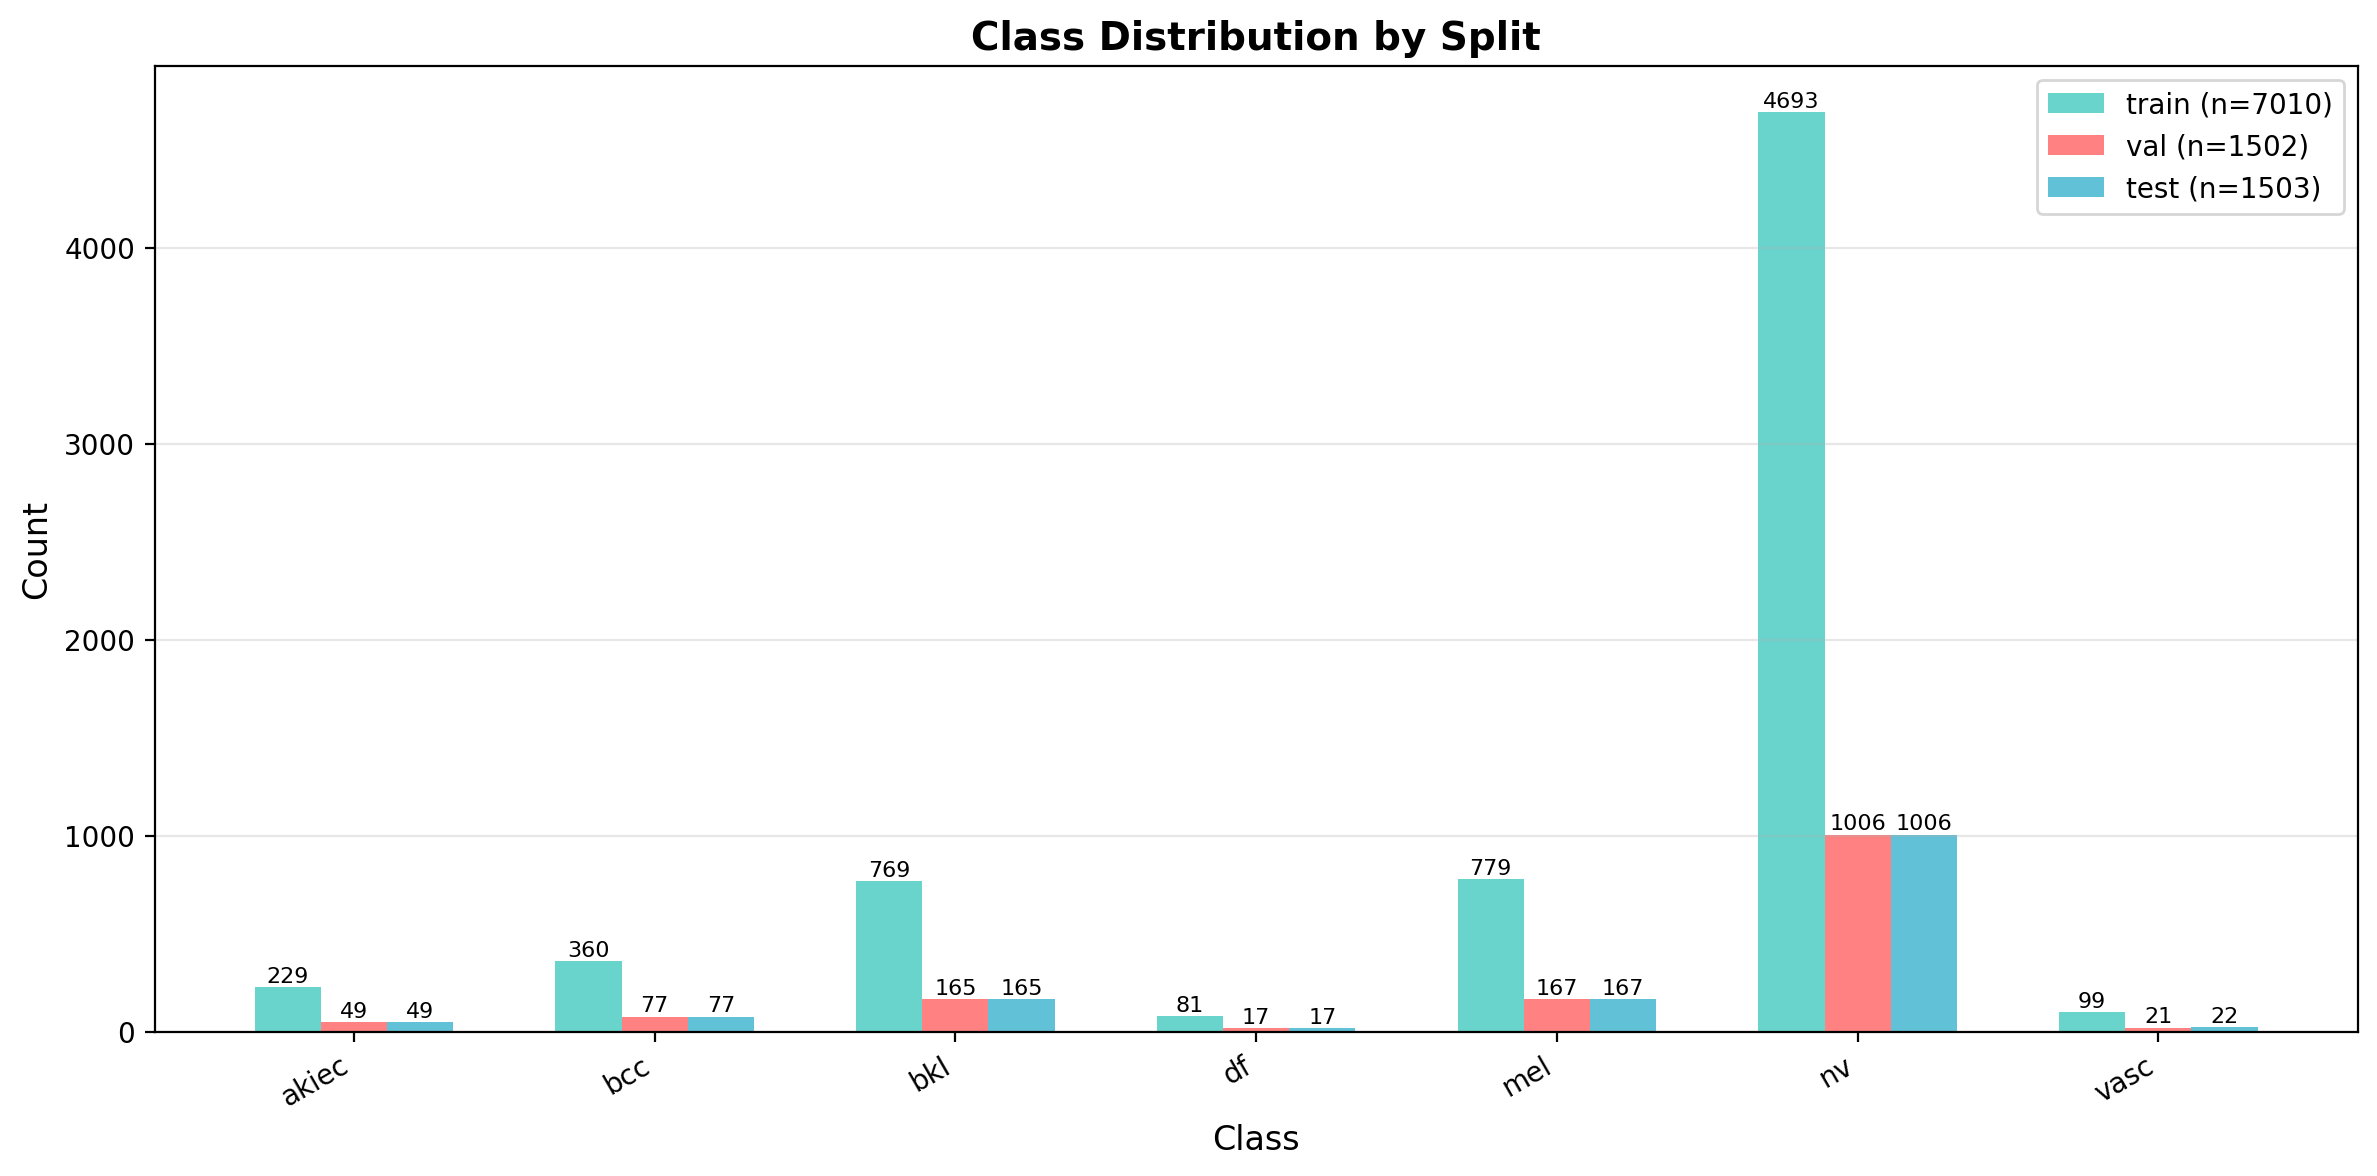
\includegraphics[width=\figwidth]{figures/class_distribution.png}
\caption{Class distribution across the training, validation, and test splits. The severe imbalance between NV and minority classes (DF, VASC) is clearly visible.}
\label{fig:class_distribution}
\end{figure}

\section{Model Architectures}

Four architectures were selected to represent a diverse spectrum of modern deep learning approaches: three CNNs and one Vision Transformer. All models were initialized with ImageNet-pretrained weights~\cite{deng2009imagenet} through the \texttt{timm} library~\cite{wightman2019timm} and fine-tuned on the ISIC 2018 dataset.

\subsection{EfficientNet-B0}

EfficientNet-B0 is the baseline model of the EfficientNet family, designed using Neural Architecture Search (NAS) and compound scaling~\cite{tan2019efficientnet}. With only 5.3 million parameters, it achieves competitive accuracy by jointly optimizing network depth, width, and resolution. In our pipeline, a dropout layer~\cite{srivastava2014dropout} ($p=0.3$) was added before the final classification head.

\subsection{ResNet50}

ResNet50 consists of 50 layers organized into four residual stages~\cite{he2016deep}. Its skip connections enable effective gradient flow during backpropagation, making it one of the most reliable architectures for transfer learning. With 25.6 million parameters, it is the second-largest model in our comparison. Dropout ($p=0.3$) was applied before the classifier.

\subsection{DenseNet121}

DenseNet121 features 121 layers with dense connectivity, where each layer receives concatenated feature maps from all preceding layers within the same dense block~\cite{huang2017densely}. This architecture promotes feature reuse and reduces parameter count to approximately 8 million. Due to the inherent regularization provided by dense connections, a slightly lower dropout ($p=0.25$) was used.

\subsection{Swin-Tiny}

Swin-Tiny is a hierarchical Vision Transformer that processes images through shifted window-based self-attention~\cite{liu2021swin}. Unlike CNNs, which rely on local receptive fields, Swin captures long-range dependencies through attention mechanisms. With 28 million parameters, it is the largest model evaluated. Following best practices for Transformer fine-tuning~\cite{touvron2021deit}, a lower learning rate ($1 \times 10^{-4}$) and higher weight decay (0.05) were used, along with an extended warmup period of 5 epochs.

\begin{table}[H]
\centering
\caption{Summary of the four evaluated architectures.}
\label{tab:architectures}
\begin{tabular}{lrllr}
\toprule
\textbf{Model} & \textbf{Params (M)} & \textbf{Type} & \textbf{Key Feature} & \textbf{Dropout} \\
\midrule
EfficientNet-B0 & 5.3  & CNN & Compound Scaling  & 0.30 \\
ResNet50        & 25.6 & CNN & Residual Connections & 0.30 \\
DenseNet121     & 8.0  & CNN & Dense Connectivity  & 0.25 \\
Swin-Tiny       & 28.0 & ViT & Shifted Window Attention & 0.30 \\
\bottomrule
\end{tabular}
\end{table}

\section{Training Pipeline}

An optimized training pipeline was developed to maximize model generalization and address the challenges of class imbalance. The pipeline integrates multiple complementary techniques, each targeting a specific aspect of the training process.

\subsection{Weighted Random Sampling}

To counteract class imbalance during training, a Weighted Random Sampler was employed. Each sample is assigned a weight inversely proportional to the frequency of its class in the training set:

\begin{equation}
w_c = \frac{N}{C \cdot n_c}
\label{eq:class_weight}
\end{equation}

where $N$ is the total number of training samples, $C$ is the number of classes, and $n_c$ is the number of samples belonging to class $c$. This ensures that mini-batches are approximately class-balanced, preventing the model from developing a bias toward the majority class (NV).

\subsection{Mixup and CutMix Augmentation}

To further regularize training and improve generalization, Mixup and CutMix were applied with equal probability ($p=0.5$ each) during training.

\textbf{Mixup} creates virtual training examples by linearly interpolating pairs of images and their labels:
\begin{equation}
\tilde{x} = \lambda x_i + (1 - \lambda) x_j, \quad \tilde{y} = \lambda y_i + (1 - \lambda) y_j
\label{eq:mixup}
\end{equation}
where $\lambda \sim \text{Beta}(\alpha, \alpha)$ with $\alpha = 0.2$.

\textbf{CutMix} replaces a rectangular patch of one image with the corresponding patch from another, adjusting the label proportionally to the area of the patch:
\begin{equation}
\tilde{x} = M \odot x_i + (1 - M) \odot x_j, \quad \tilde{y} = \lambda y_i + (1 - \lambda) y_j
\label{eq:cutmix}
\end{equation}
where $M$ is a binary mask indicating the cut region and $\lambda$ equals the ratio of the unmasked area. The CutMix alpha was set to 1.0.

These augmentations force the model to learn from mixed signals, discouraging memorization and encouraging smoother decision boundaries.

\subsection{Label Smoothing}

Standard one-hot encoded labels assign a probability of 1.0 to the correct class and 0.0 to all others. Label Smoothing redistributes a small fraction of the probability mass to incorrect classes:
\begin{equation}
y_{\text{smooth}} = (1 - \epsilon) \cdot y_{\text{one-hot}} + \frac{\epsilon}{C}
\label{eq:label_smooth}
\end{equation}
where $\epsilon = 0.1$ is the smoothing factor and $C = 7$ is the number of classes. This technique prevents the model from becoming overconfident in its predictions, which improves calibration and AUC scores.

\subsection{Optimization and Scheduling}

All models were trained using the AdamW optimizer~\cite{loshchilov2019decoupled}, which decouples weight decay from the gradient update, leading to better generalization compared to standard Adam. A cosine annealing schedule with linear warmup~\cite{loshchilov2017sgdr} was employed:

\begin{itemize}
    \item \textbf{Warmup phase} (first 3--5 epochs): The learning rate increases linearly from a near-zero value to the target learning rate, preventing early instability when the randomly initialized classification head produces large gradients.
    \item \textbf{Cosine decay phase} (remaining epochs): The learning rate decreases following a cosine curve to a minimum value of $1 \times 10^{-6}$, allowing the model to settle into a flat minimum of the loss landscape.
\end{itemize}

\subsection{Data Augmentation}

Beyond Mixup and CutMix, the following standard augmentations were applied during training:
\begin{itemize}
    \item Random horizontal and vertical flips ($p=0.5$)
    \item Random rotation (up to $\pm90^\circ$)
    \item Color jittering (brightness, contrast, saturation, hue; magnitude 0.25)
    \item Random Resized Crop (scale range: 0.85--1.0)
    \item Gaussian Blur ($p=0.1$)
    \item Random Erasing ($p=0.1$)
\end{itemize}

All images were resized to $224 \times 224$ pixels and normalized using ImageNet mean and standard deviation values~\cite{deng2009imagenet}. A batch size of 16 was selected to accommodate GPU memory constraints when running all four architectures (including the 28M-parameter Swin-Tiny) under identical conditions with mixed-precision training, ensuring a fair and consistent comparison across all experiments.

\begin{table}[H]
\centering
\caption{Hyperparameter configuration for each model.}
\label{tab:hyperparams}
\begin{tabular}{lcccc}
\toprule
\textbf{Hyperparameter} & \textbf{EB0} & \textbf{RN50} & \textbf{DN121} & \textbf{Swin-T} \\
\midrule
Learning Rate        & 3e-4  & 3e-4  & 2.5e-4 & 1e-4 \\
Weight Decay         & 1e-3  & 1e-3  & 1e-3   & 5e-2 \\
Warmup Epochs        & 3     & 3     & 3      & 5 \\
Max Epochs           & 50    & 50    & 50     & 50 \\
Batch Size           & 16    & 16    & 16     & 16 \\
Early Stopping       & 12    & 12    & 12     & 12 \\
Mixup $\alpha$       & 0.2   & 0.2   & 0.2    & 0.2 \\
CutMix $\alpha$      & 1.0   & 1.0   & 1.0    & 1.0 \\
Label Smoothing      & 0.1   & 0.1   & 0.1    & 0.1 \\
\bottomrule
\end{tabular}
\end{table}

\section{Evaluation Metrics}

Given the severe class imbalance, accuracy alone is an insufficient measure of model performance. A model that simply predicts NV for every input would achieve approximately 67\% accuracy. Therefore, we report a comprehensive set of metrics:

\begin{itemize}
    \item \textbf{Macro F1-Score:} The unweighted mean of per-class F1-scores, giving equal importance to all classes regardless of their frequency. This is our primary selection metric.
    \item \textbf{Area Under the ROC Curve (AUC):} Measures the model's ability to discriminate between classes across all possible decision thresholds. A macro-averaged AUC close to 1.0 indicates excellent probability calibration.
    \item \textbf{Cohen's Kappa ($\kappa$):} Measures agreement between predicted and true labels, correcting for chance agreement. Values above 0.6 indicate substantial agreement.
    \item \textbf{Matthews Correlation Coefficient (MCC):} A balanced measure that accounts for all four entries of the confusion matrix (TP, TN, FP, FN), considered the most informative single metric for imbalanced classification.
    \item \textbf{Per-class Sensitivity and Specificity:} Sensitivity (recall) measures the proportion of actual positives correctly identified, while specificity measures the proportion of actual negatives correctly identified. Both are critical in medical diagnostics.
\end{itemize}

\section{Ensemble Strategy}

After training all four models independently, we constructed an ensemble using soft voting. For each test sample, the softmax probability vectors from all four models were averaged element-wise, and the final prediction was taken as the class with the highest averaged probability:

\begin{equation}
\hat{y} = \arg\max_c \frac{1}{M} \sum_{m=1}^{M} p_m(c \mid x)
\label{eq:ensemble}
\end{equation}

where $M=4$ is the number of models and $p_m(c \mid x)$ is the probability assigned to class $c$ by model $m$. This approach leverages the complementary strengths of different architectures: CNNs provide strong local feature extraction while the Transformer captures global spatial relationships.

\section{Model Interpretability with Grad-CAM}

To ensure that the trained models attend to clinically meaningful regions, Gradient-weighted Class Activation Mapping (Grad-CAM)~\cite{selvaraju2017grad} was applied. Given a target class $c$, Grad-CAM computes the gradient of the class score $y^c$ with respect to the feature maps $A^k$ of the last convolutional layer:

\begin{equation}
\alpha_k^c = \frac{1}{Z} \sum_i \sum_j \frac{\partial y^c}{\partial A_{ij}^k}
\label{eq:gradcam_weights}
\end{equation}

The final heatmap is obtained by computing a weighted combination of the feature maps followed by a ReLU activation:

\begin{equation}
L_{\text{Grad-CAM}}^c = \text{ReLU}\left(\sum_k \alpha_k^c A^k\right)
\label{eq:gradcam}
\end{equation}

This produces a coarse localization map highlighting regions that positively influence the prediction for class $c$. The heatmap is then upsampled to the input image resolution and overlaid as a color-coded visualization.

% ======================= CHAPTER 4: EXPERIMENTS AND RESULTS ==========================
\chapter{Experiments and Results}

This chapter presents the experimental results of our study. We first compare the four individual models, then analyze the ensemble approach, followed by Grad-CAM visualizations and the ablation study.

All experiments were conducted on a single NVIDIA GPU using mixed-precision training (FP16) with PyTorch 2.x. The random seed was fixed at 42 for reproducibility.

\section{Individual Model Comparison}

\subsection{Overall Performance}

Table~\ref{tab:model_comparison} summarizes the test-set performance of all four architectures trained with the optimized pipeline.

\begin{table}[H]
\centering
\caption{Test-set performance comparison of the four evaluated architectures. Best values are highlighted in \textbf{bold}.}
\label{tab:model_comparison}
\begin{tabular}{lccccc}
\toprule
\textbf{Model} & \textbf{Accuracy} & \textbf{Macro F1} & \textbf{AUC} & \textbf{MCC} & \textbf{Kappa} \\
\midrule
EfficientNet-B0 & \textbf{0.8836} & \textbf{0.8311} & 0.9522 & \textbf{0.7721} & \textbf{0.7710} \\
ResNet50        & 0.8603 & 0.7902 & 0.9565 & 0.7310 & 0.7309 \\
DenseNet121     & 0.8543 & 0.7967 & 0.9587 & 0.7209 & 0.7206 \\
Swin-Tiny       & 0.8490 & 0.7855 & \textbf{0.9600} & 0.7157 & 0.7150 \\
\bottomrule
\end{tabular}
\end{table}

EfficientNet-B0 achieved the highest accuracy (88.36\%) and macro F1-score (0.831) among all individual models, despite being the smallest architecture with only 5.3M parameters. This result underscores the effectiveness of compound scaling~\cite{tan2019efficientnet}: EfficientNet achieves superior feature extraction with significantly fewer parameters than ResNet50 (25.6M) or Swin-Tiny (28M).\footnote{The relatively high test cross-entropy loss (0.75) observed for all models is an expected artifact of label smoothing training~\cite{muller2019does}: since the models are trained with soft targets ($\epsilon=0.1$), they learn to output maximum confidence $\approx 1 - \epsilon + \epsilon/C \approx 0.93$ rather than 1.0, resulting in higher raw loss values that do not reflect degraded classification quality.}

An intriguing pattern emerges when comparing accuracy against AUC. While EfficientNet-B0 leads in hard-classification metrics (accuracy, F1), Swin-Tiny achieves the highest AUC (0.960). This suggests that the self-attention mechanism of Transformers~\cite{dosovitskiy2021image} produces better-calibrated probability distributions, even though its discrete classification decisions are slightly less accurate on this relatively small dataset. This finding is consistent with the literature suggesting that Vision Transformers require larger datasets to fully exploit their modeling capacity~\cite{touvron2021deit}.

\subsection{Per-Class Analysis}

Table~\ref{tab:per_class_f1} presents the per-class F1-scores and AUC values for each model.

\begin{table}[H]
\centering
\caption{Per-class F1-scores and AUC values for each model on the test set.}
\label{tab:per_class_f1}
\begin{tabular}{l|cc|cc|cc|cc}
\toprule
\textbf{Class} & \multicolumn{2}{c|}{\textbf{EB0}} & \multicolumn{2}{c|}{\textbf{RN50}} & \multicolumn{2}{c|}{\textbf{DN121}} & \multicolumn{2}{c}{\textbf{Swin-T}} \\
 & F1 & AUC & F1 & AUC & F1 & AUC & F1 & AUC \\
\midrule
AKIEC & \textbf{0.717} & 0.921 & 0.646 & \textbf{0.949} & 0.637 & 0.928 & 0.660 & 0.949 \\
BCC   & \textbf{0.865} & \textbf{0.984} & 0.837 & 0.977 & 0.815 & 0.989 & 0.800 & 0.993 \\
BKL   & \textbf{0.758} & \textbf{0.938} & 0.730 & 0.926 & 0.741 & 0.945 & 0.698 & 0.947 \\
DF    & \textbf{0.938} & 0.963 & 0.800 & 0.981 & 0.867 & \textbf{0.992} & 0.914 & 0.942 \\
MEL   & \textbf{0.695} & 0.913 & 0.634 & 0.922 & 0.642 & 0.922 & 0.625 & \textbf{0.930} \\
NV    & \textbf{0.940} & 0.946 & 0.929 & 0.944 & 0.920 & 0.946 & 0.921 & \textbf{0.960} \\
VASC  & 0.905 & \textbf{1.000} & \textbf{0.955} & 0.997 & \textbf{0.955} & 0.989 & 0.880 & \textbf{1.000} \\
\bottomrule
\end{tabular}
\end{table}

Several important observations can be drawn from this per-class analysis:

\textbf{Melanoma (MEL)} remains the most challenging class across all models, with F1-scores ranging from 0.625 (Swin-Tiny) to 0.695 (EfficientNet-B0). This difficulty arises from melanoma's morphological overlap with benign keratosis (BKL) and melanocytic nevi (NV). However, melanoma AUC values range from 0.913 to 0.930, indicating that models can rank melanoma cases with reasonable confidence even when the hard classification threshold is suboptimal.

\textbf{Dermatofibroma (DF)} achieves remarkably high F1-scores (0.800--0.938) despite being the rarest class with only 17 test samples. This suggests that DF has distinctive visual features that are well-captured by transfer learning, and that the Weighted Random Sampler effectively compensates for its scarcity. However, these results should be interpreted with caution: with only 17 test samples, a single additional misclassification would reduce the F1-score by approximately 0.06, making these estimates sensitive to individual predictions.

\textbf{Vascular Lesion (VASC)} is consistently well-classified, with F1-scores between 0.880 and 0.955 and near-perfect AUC values (similarly based on a small test set of 22 samples). The distinctive red-purple coloration of vascular lesions provides strong discriminative signals for all architectures.

\subsection{Training Dynamics}

Figure~\ref{fig:training_history} shows the training and validation loss curves for all four models. All models demonstrate healthy convergence without significant overfitting, validating the effectiveness of the combined regularization strategy (Mixup + CutMix + Label Smoothing + Weight Decay).

\begin{figure}[H]
\centering
\begin{subfigure}{\textwidth}
    \makebox[\textwidth][c]{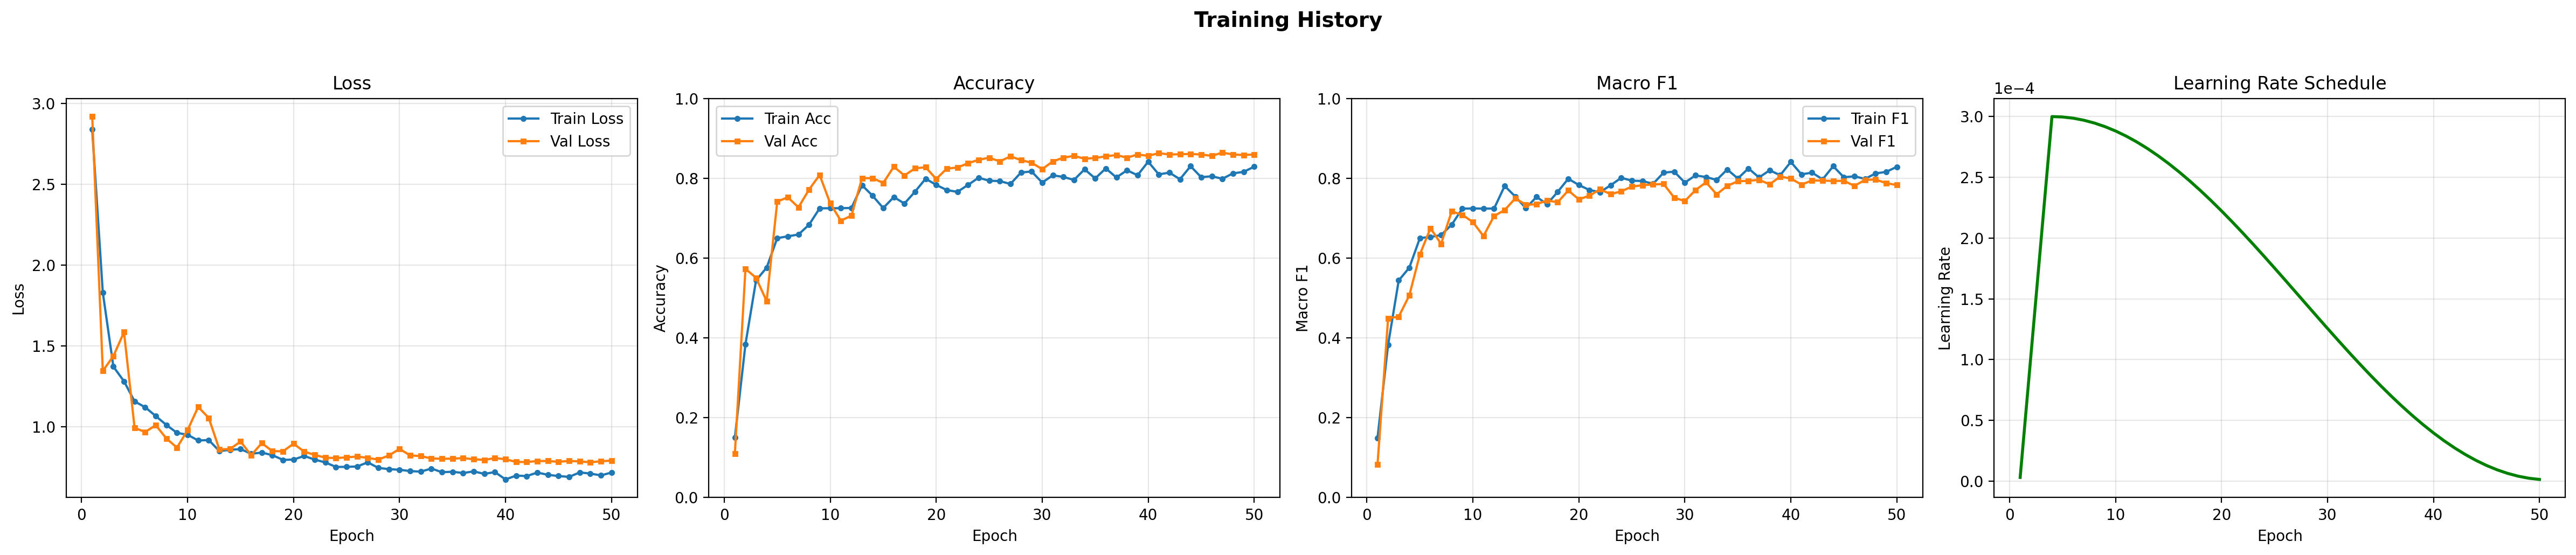
\includegraphics[width=1.15\textwidth]{figures/eb0_training_history.png}}
    \caption{EfficientNet-B0}
\end{subfigure}

\vspace{0.6cm}

\begin{subfigure}{\textwidth}
    \makebox[\textwidth][c]{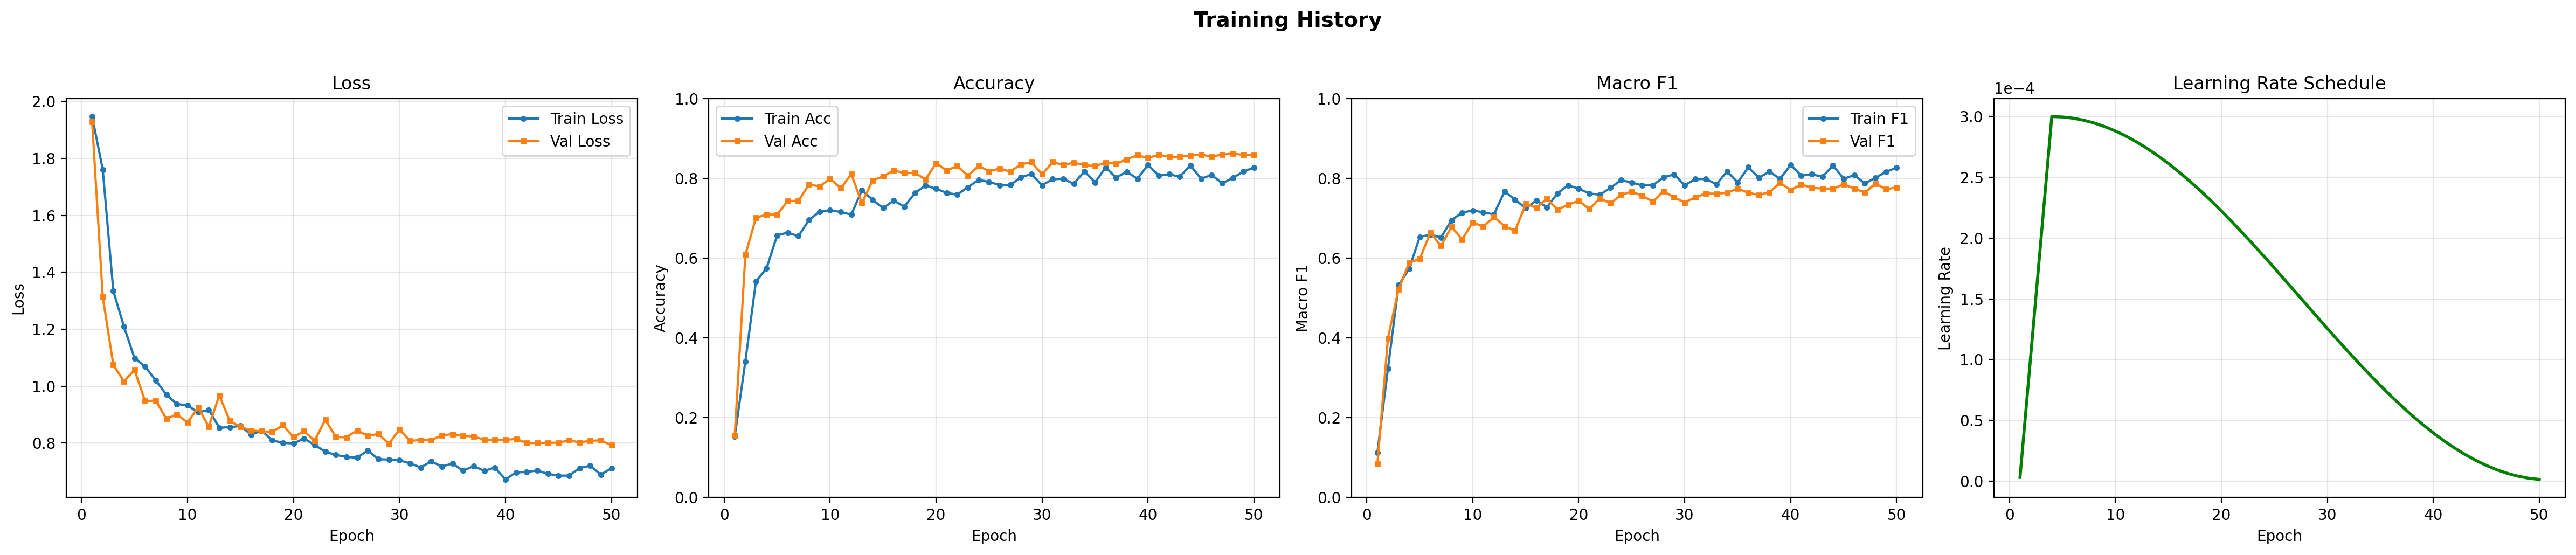
\includegraphics[width=1.15\textwidth]{figures/rn50_training_history.png}}
    \caption{ResNet50}
\end{subfigure}
\caption{Training history for all four models, showing loss, accuracy, and learning rate progression across epochs. All models demonstrate stable convergence without overfitting.}
\label{fig:training_history}
\end{figure}

\begin{figure}[H]
\ContinuedFloat
\centering
\begin{subfigure}{\textwidth}
    \makebox[\textwidth][c]{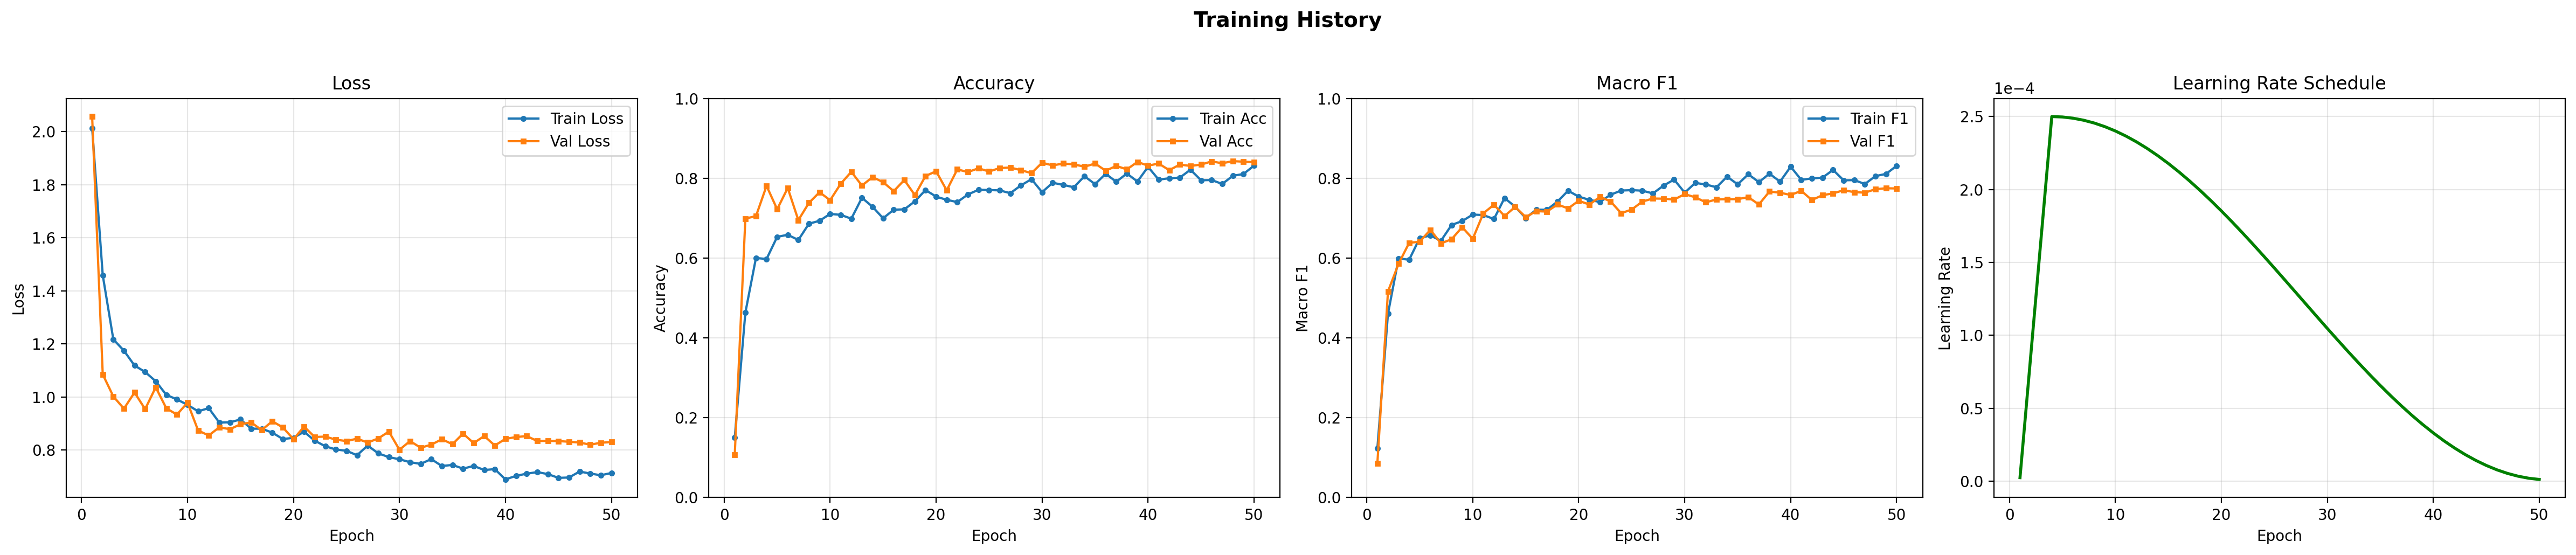
\includegraphics[width=1.15\textwidth]{figures/dn121_training_history.png}}
    \caption{DenseNet121}
\end{subfigure}

\vspace{0.6cm}

\begin{subfigure}{\textwidth}
    \makebox[\textwidth][c]{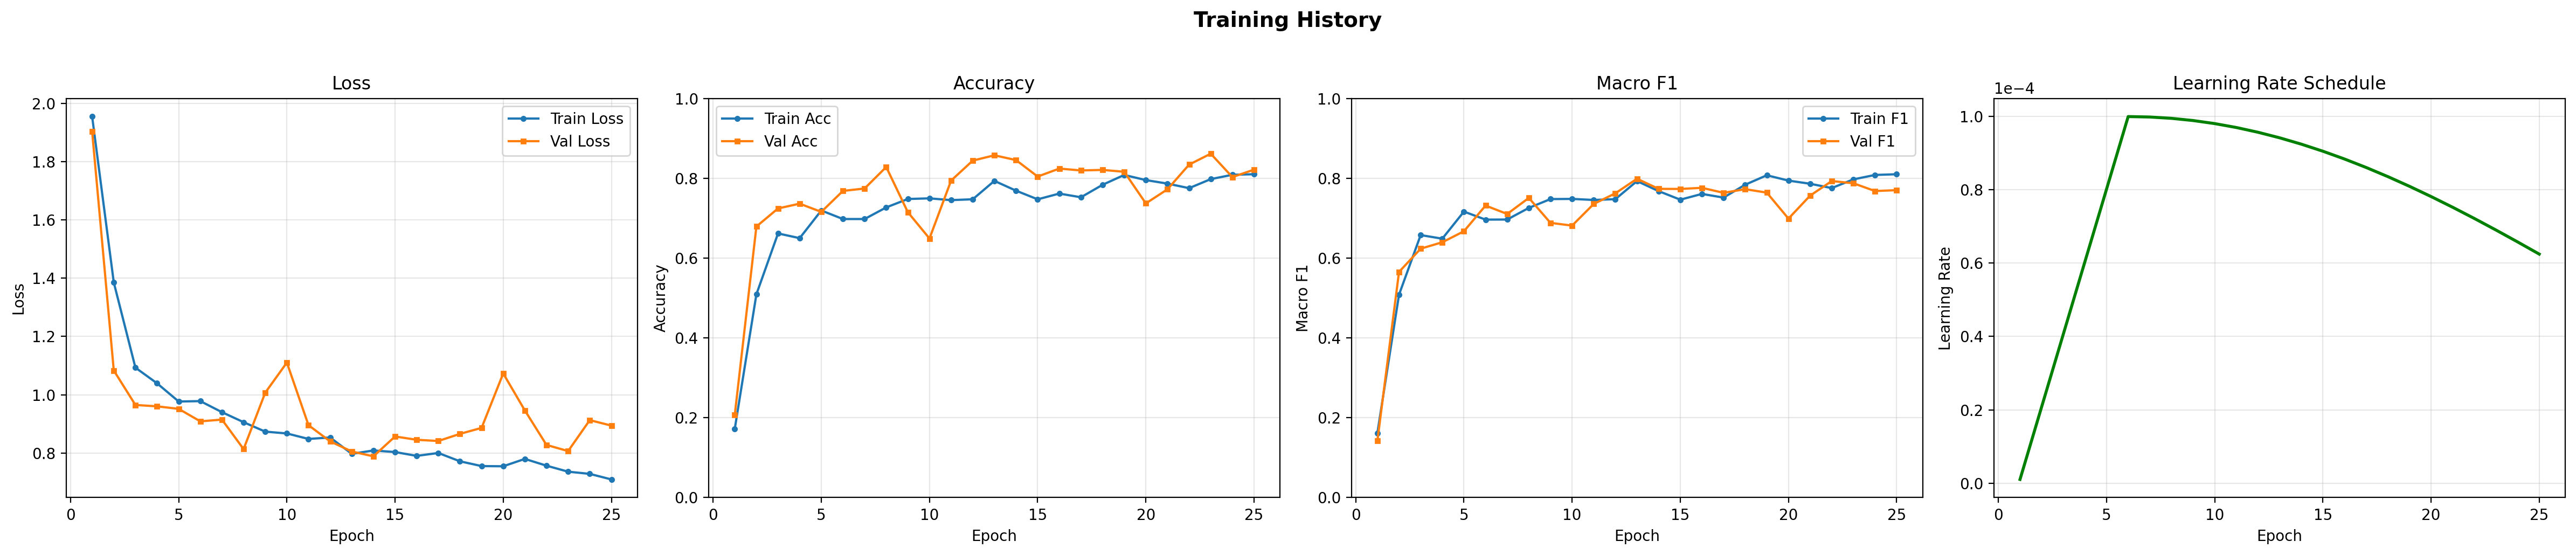
\includegraphics[width=1.15\textwidth]{figures/swin_training_history.png}}
    \caption{Swin-Tiny}
\end{subfigure}
\caption[]{Training history for all four models (continued).}
\end{figure}

Notable differences in convergence behavior include:
\begin{itemize}
    \item \textbf{EfficientNet-B0 and ResNet50} both achieved their best validation performance at epoch 39, with 11 subsequent epochs showing no improvement.
    \item \textbf{DenseNet121} reached its best performance at epoch 49 out of 50, suggesting that the dense connectivity pattern requires more training iterations to fully converge.
    \item \textbf{Swin-Tiny} triggered early stopping at epoch 25 (best at epoch 13), indicating faster convergence but also a tendency to overfit earlier than the CNN models on this relatively small dataset.
\end{itemize}

\subsection{Confusion Matrices}

Figure~\ref{fig:confusion_matrices} presents the normalized confusion matrices for all four models. The most common misclassification pattern across all models is the confusion between MEL and NV, which is clinically expected given their morphological similarity. BKL is also frequently confused with NV.

\begin{figure}[H]
\centering
\begin{subfigure}{\textwidth}
    \makebox[\textwidth][c]{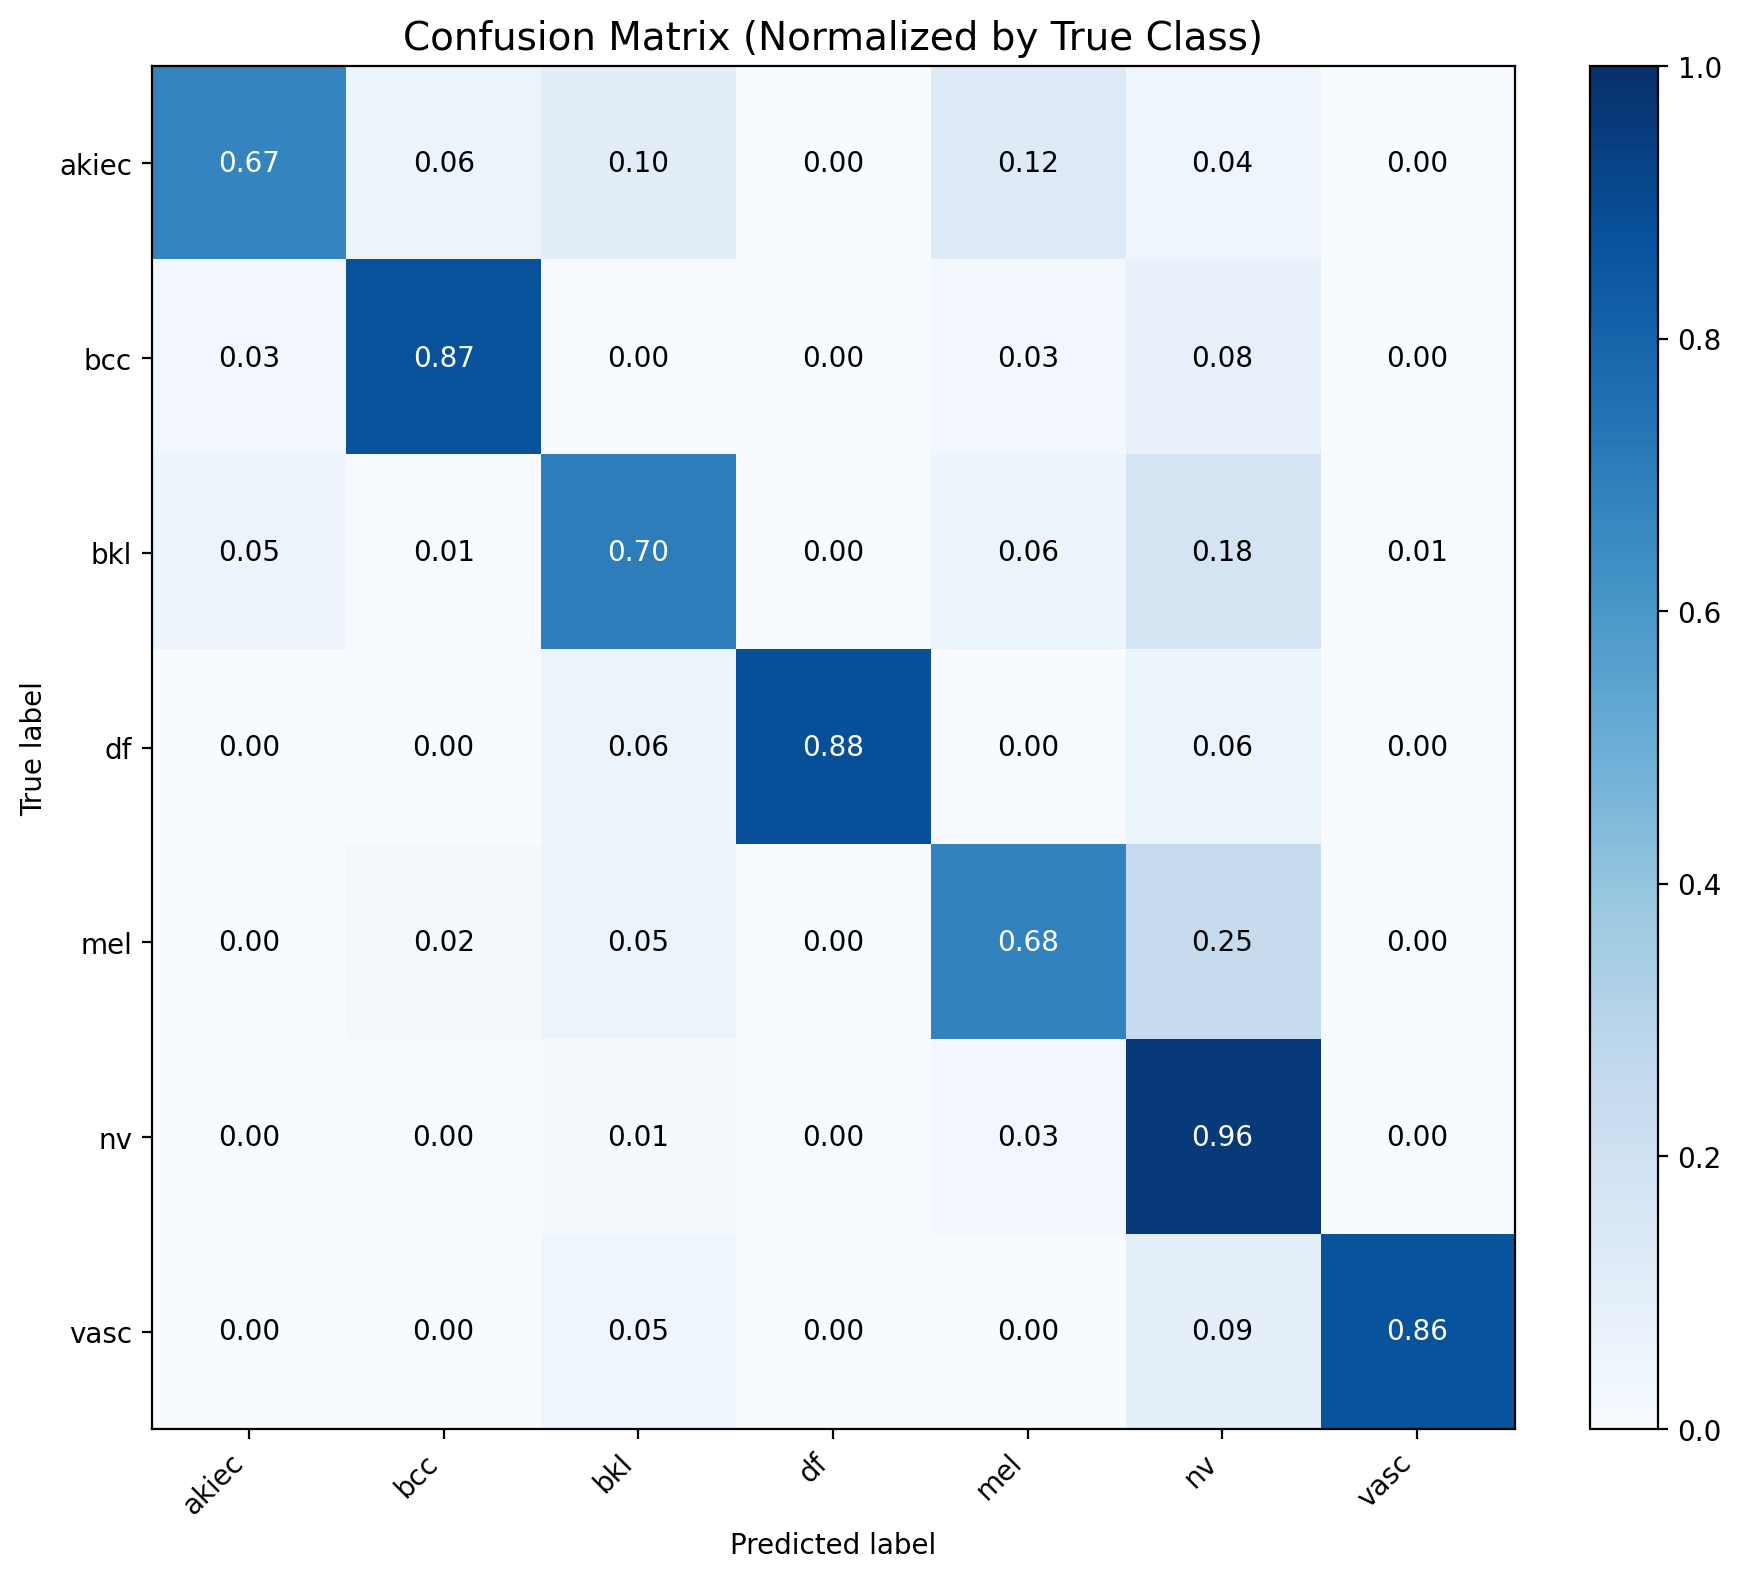
\includegraphics[width=0.9\textwidth]{figures/eb0_confusion_matrix.png}}
    \caption{EfficientNet-B0}
\end{subfigure}

\vspace{0.6cm}

\begin{subfigure}{\textwidth}
    \makebox[\textwidth][c]{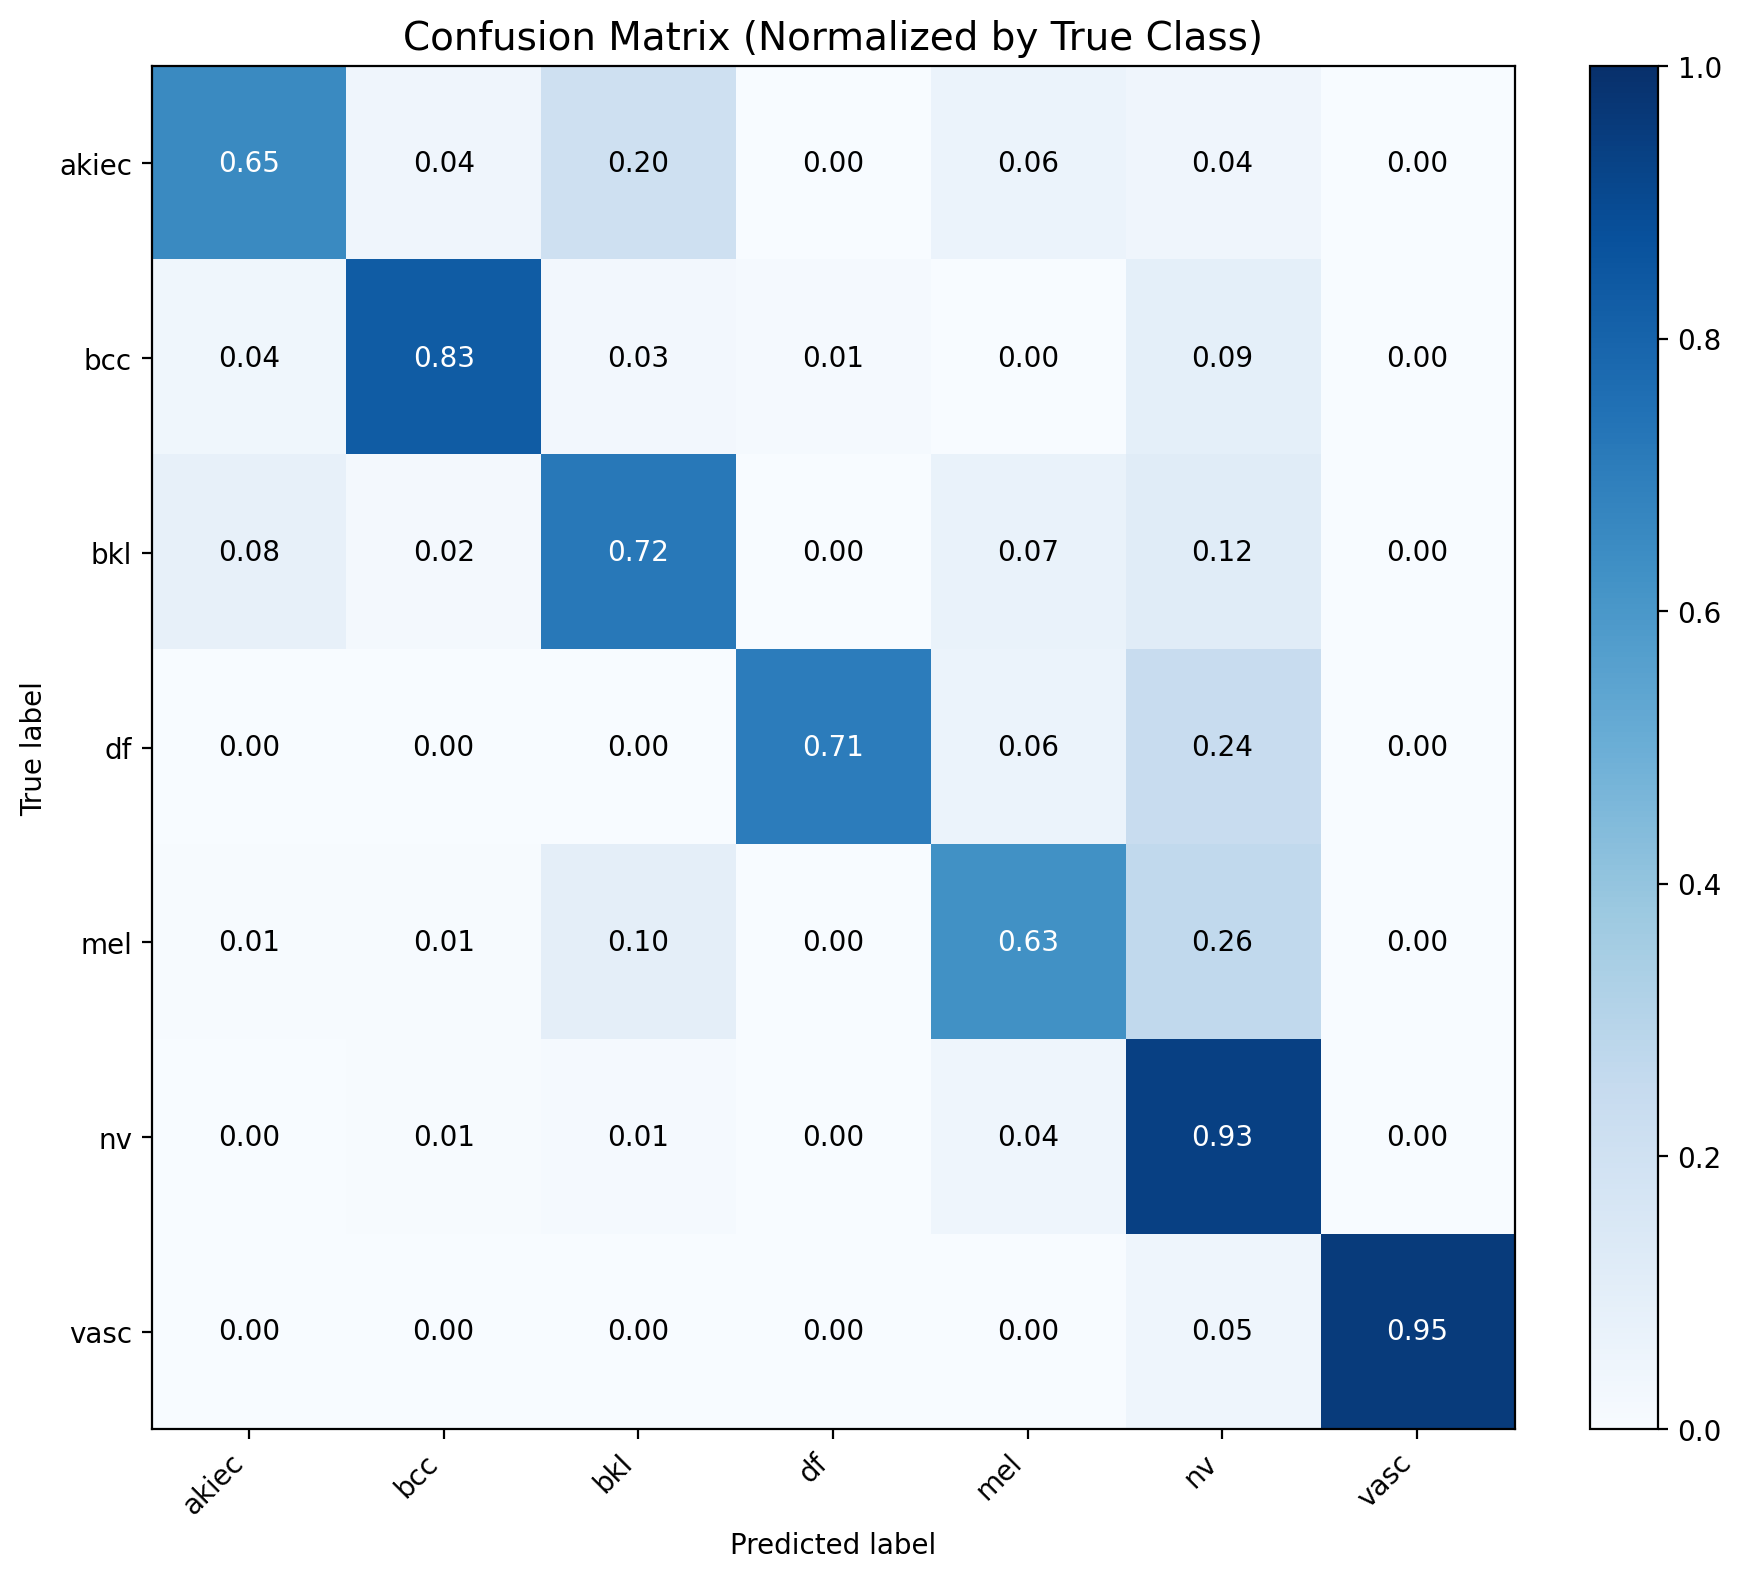
\includegraphics[width=0.9\textwidth]{figures/rn50_confusion_matrix.png}}
    \caption{ResNet50}
\end{subfigure}
\caption{Normalized confusion matrices for all four models on the test set.}
\label{fig:confusion_matrices}
\end{figure}

\begin{figure}[H]
\ContinuedFloat
\centering
\begin{subfigure}{\textwidth}
    \makebox[\textwidth][c]{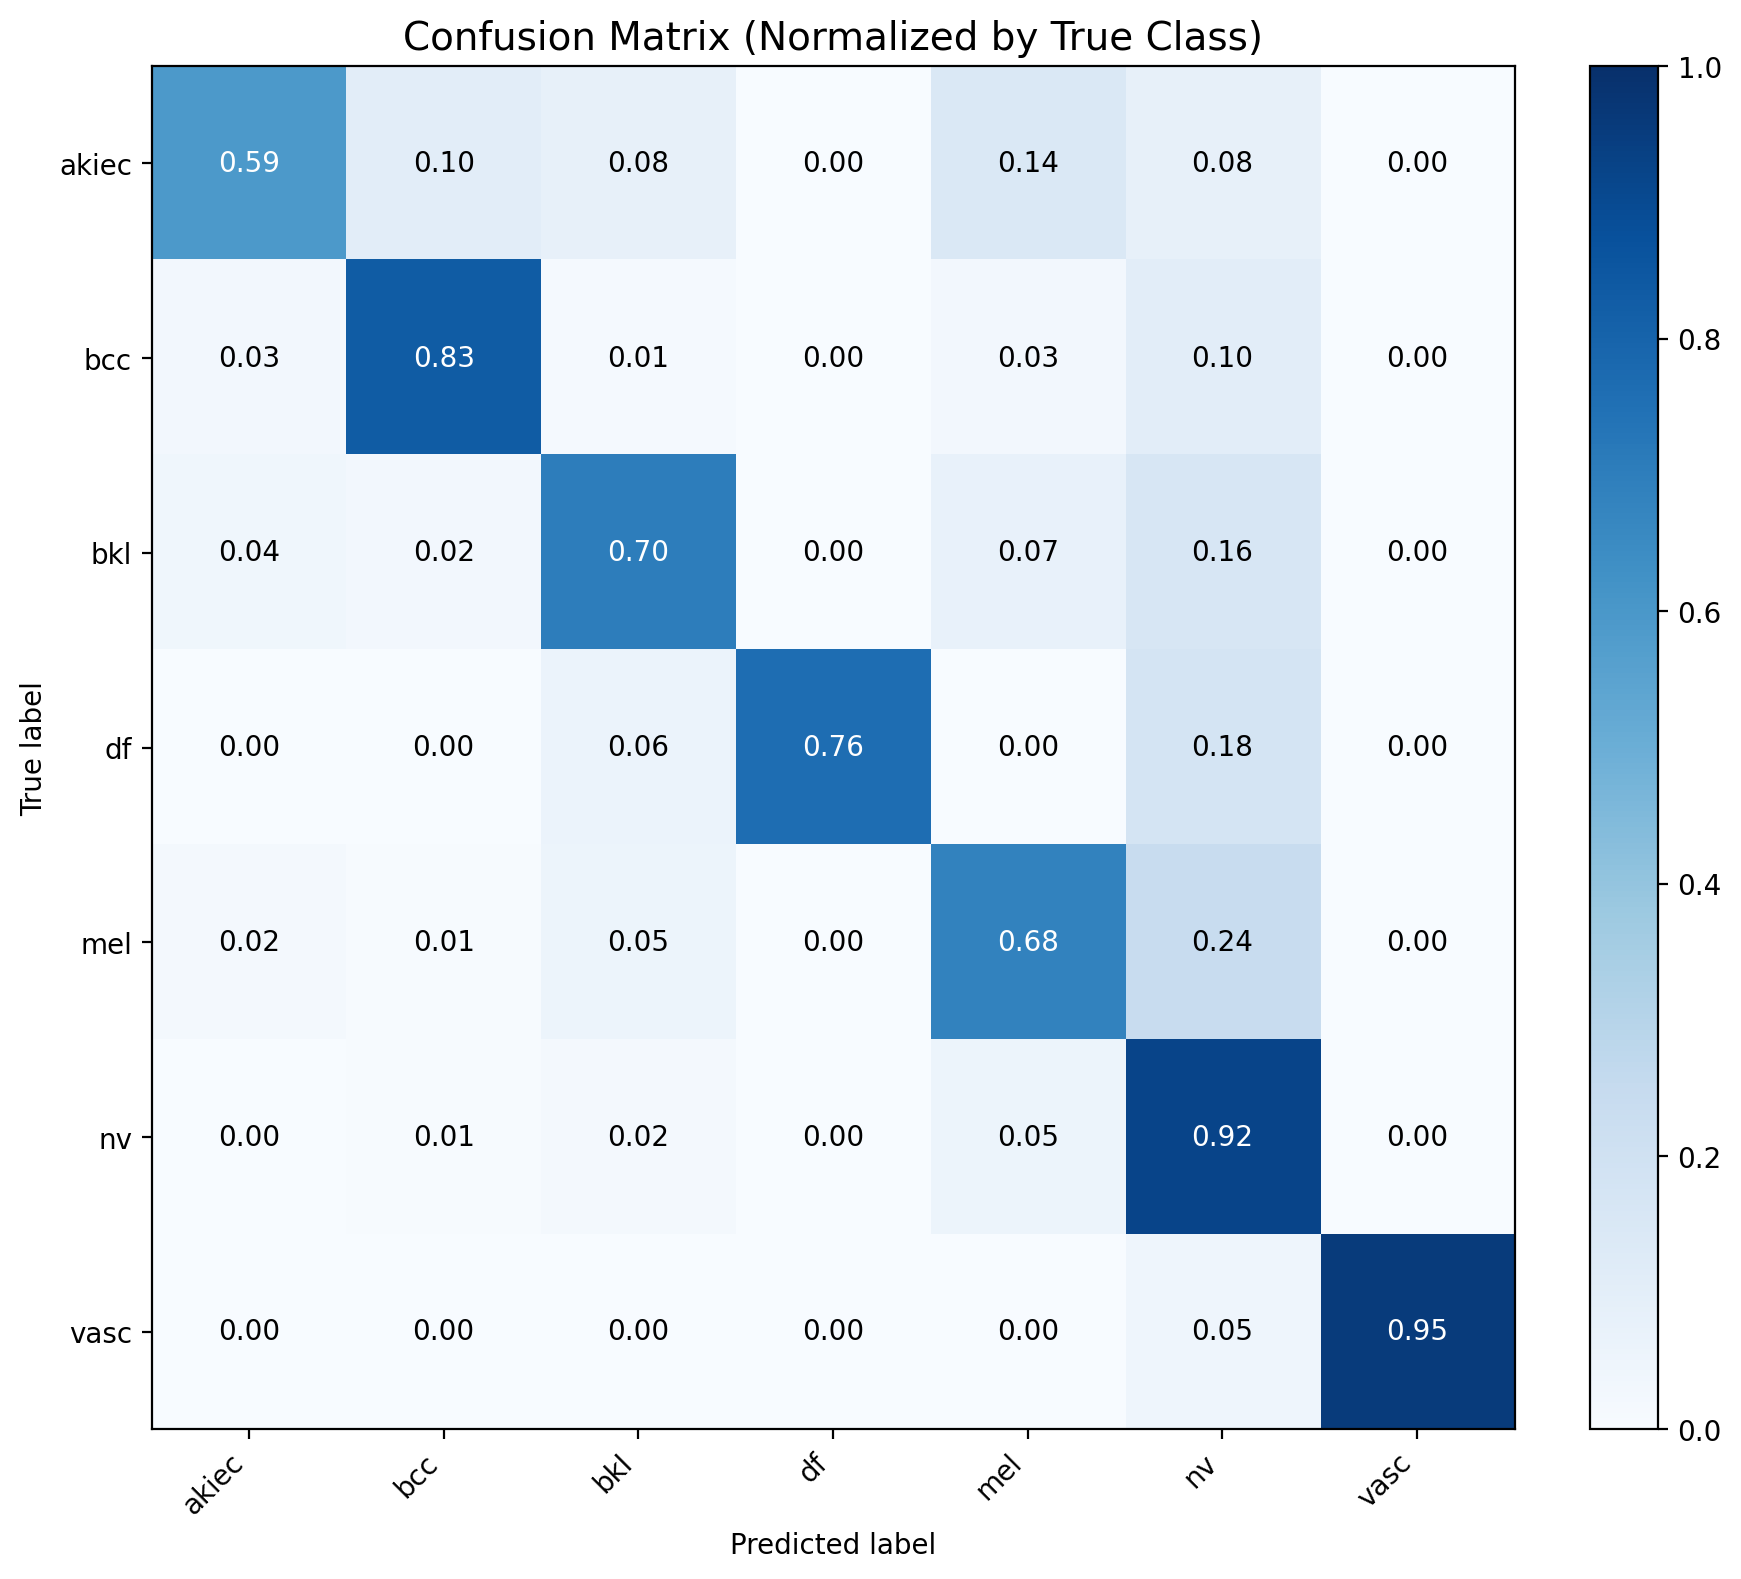
\includegraphics[width=0.9\textwidth]{figures/dn121_confusion_matrix.png}}
    \caption{DenseNet121}
\end{subfigure}

\vspace{0.6cm}

\begin{subfigure}{\textwidth}
    \makebox[\textwidth][c]{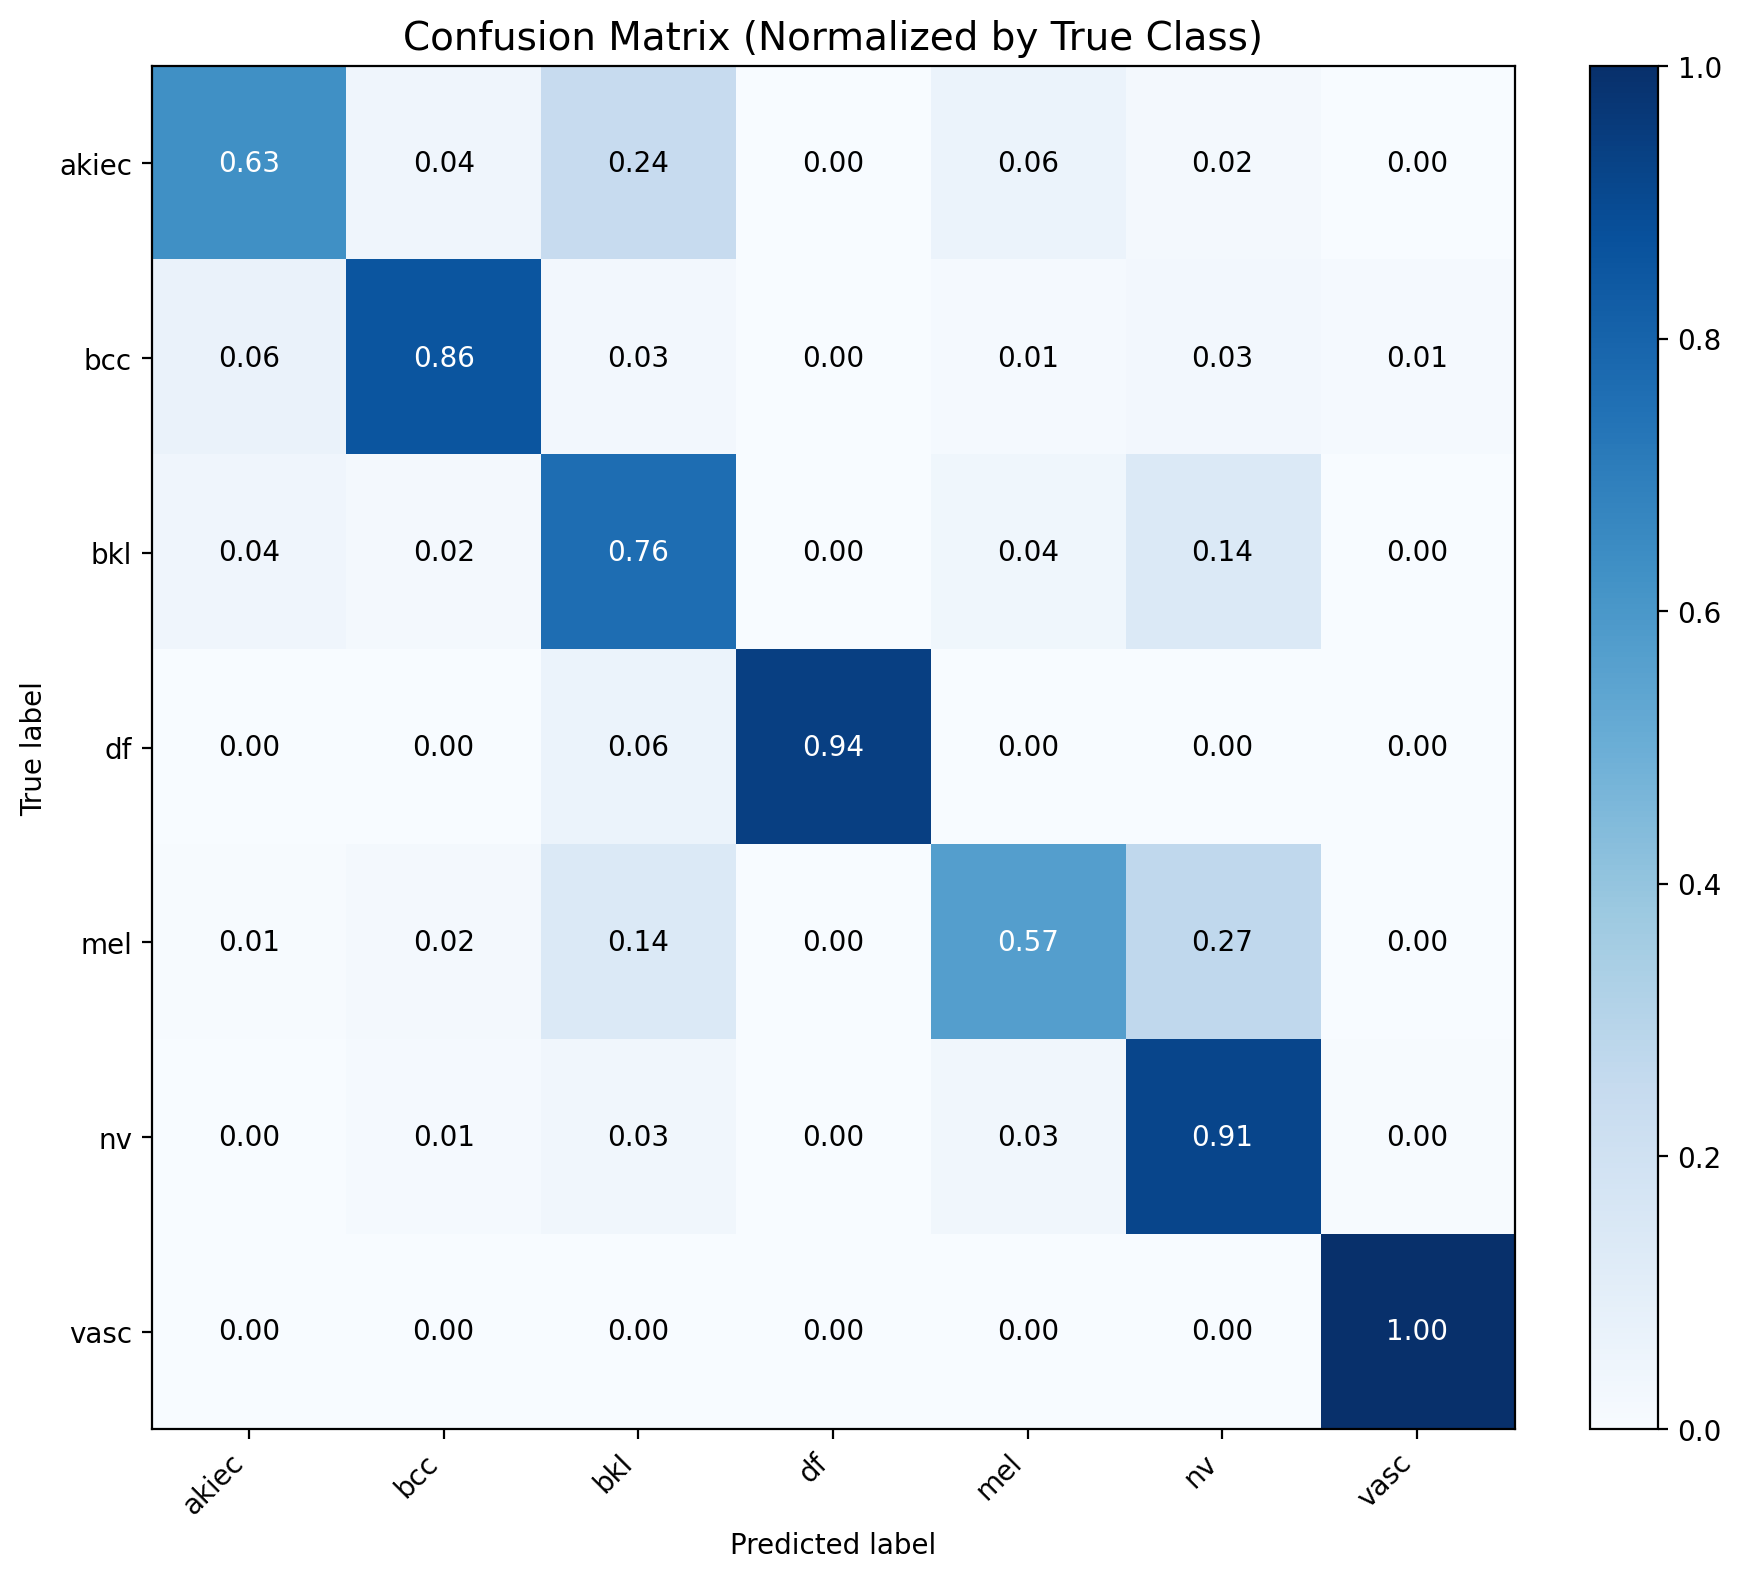
\includegraphics[width=0.9\textwidth]{figures/swin_confusion_matrix.png}}
    \caption{Swin-Tiny}
\end{subfigure}
\caption[]{Normalized confusion matrices for all four models on the test set (continued).}
    \end{figure}


    \section{Ensemble Results}

A soft-voting ensemble~\cite{ganaie2022ensemble} combining all four models achieved the best overall performance, as shown in Table~\ref{tab:ensemble_results}.

\begin{table}[H]
\centering
\caption{Comparison of individual models versus the ensemble on the test set.}
\label{tab:ensemble_results}
\begin{tabular}{lccccc}
\toprule
\textbf{Model} & \textbf{Accuracy} & \textbf{Macro F1} & \textbf{AUC} & \textbf{MCC} & \textbf{Kappa} \\
\midrule
EfficientNet-B0  & 0.8836 & 0.8311 & 0.9522 & 0.7721 & 0.7710 \\
ResNet50         & 0.8603 & 0.7902 & 0.9565 & 0.7310 & 0.7309 \\
DenseNet121      & 0.8543 & 0.7967 & 0.9587 & 0.7209 & 0.7206 \\
Swin-Tiny        & 0.8490 & 0.7855 & 0.9600 & 0.7157 & 0.7150 \\
\midrule
\textbf{Ensemble (4 models)} & \textbf{0.8949} & \textbf{0.8446} & \textbf{0.9802} & \textbf{0.7956} & \textbf{0.7949} \\
\bottomrule
\end{tabular}
\end{table}

The ensemble improved accuracy by +1.13\% over the best individual model (EfficientNet-B0) and, more importantly, boosted the macro AUC from 0.952 to \textbf{0.980}---a substantial improvement indicating near-perfect probability calibration across all classes. The melanoma F1-score improved from 0.695 to 0.744 (+4.9\%), demonstrating that architectural diversity helps reduce class-specific errors.

\begin{figure}[H]
\centering
\begin{subfigure}{0.46\textwidth}
    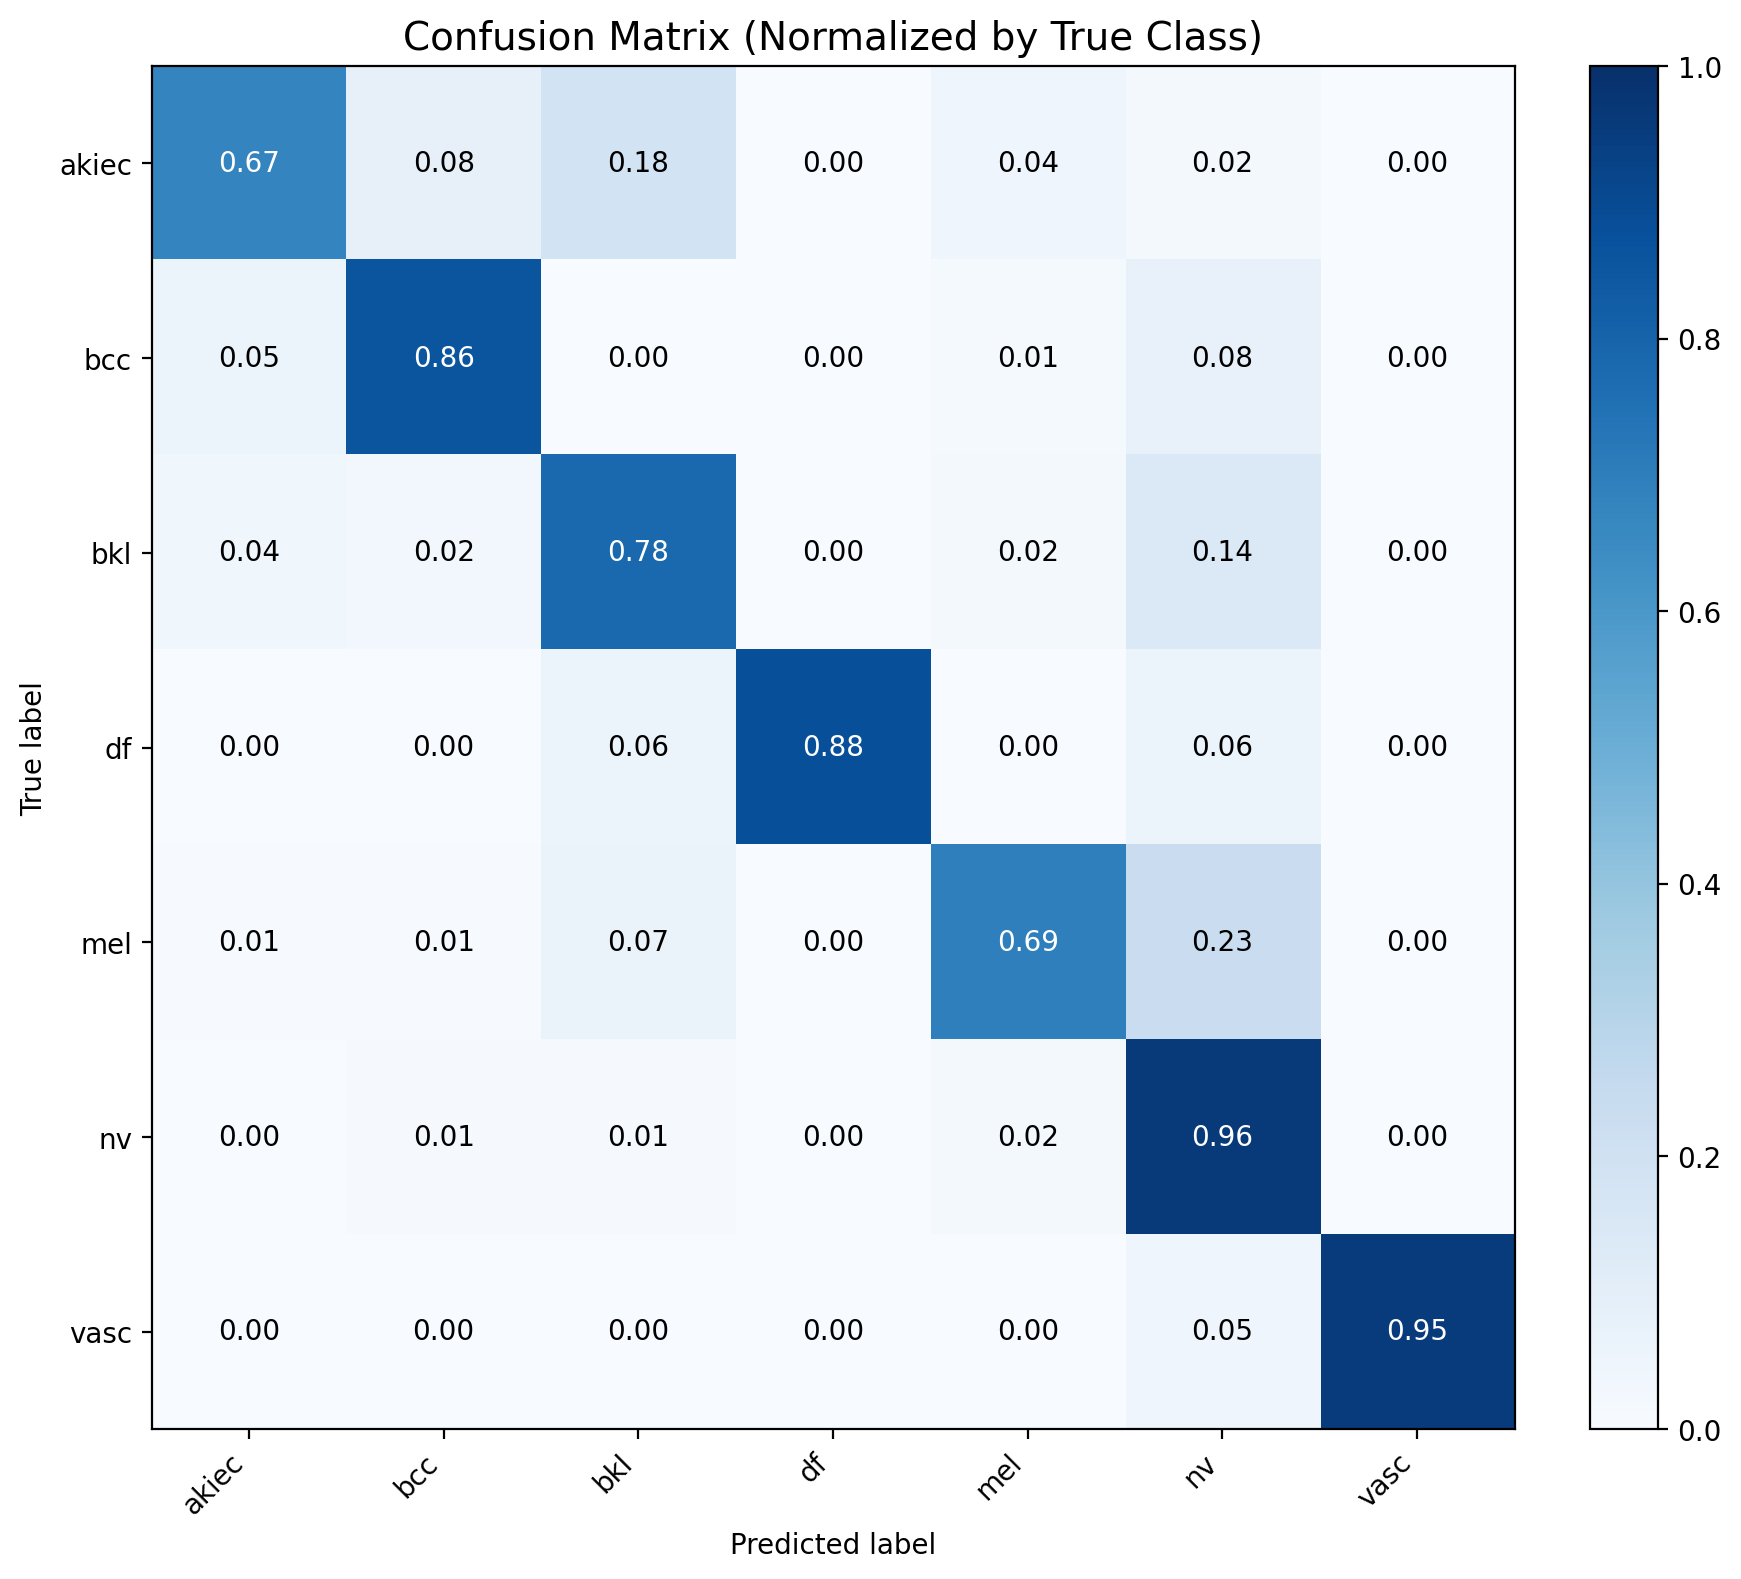
\includegraphics[width=\textwidth]{figures/ensemble_confusion_matrix.png}
    \caption{Confusion matrix}
\end{subfigure}
\hfill
\begin{subfigure}{0.46\textwidth}
    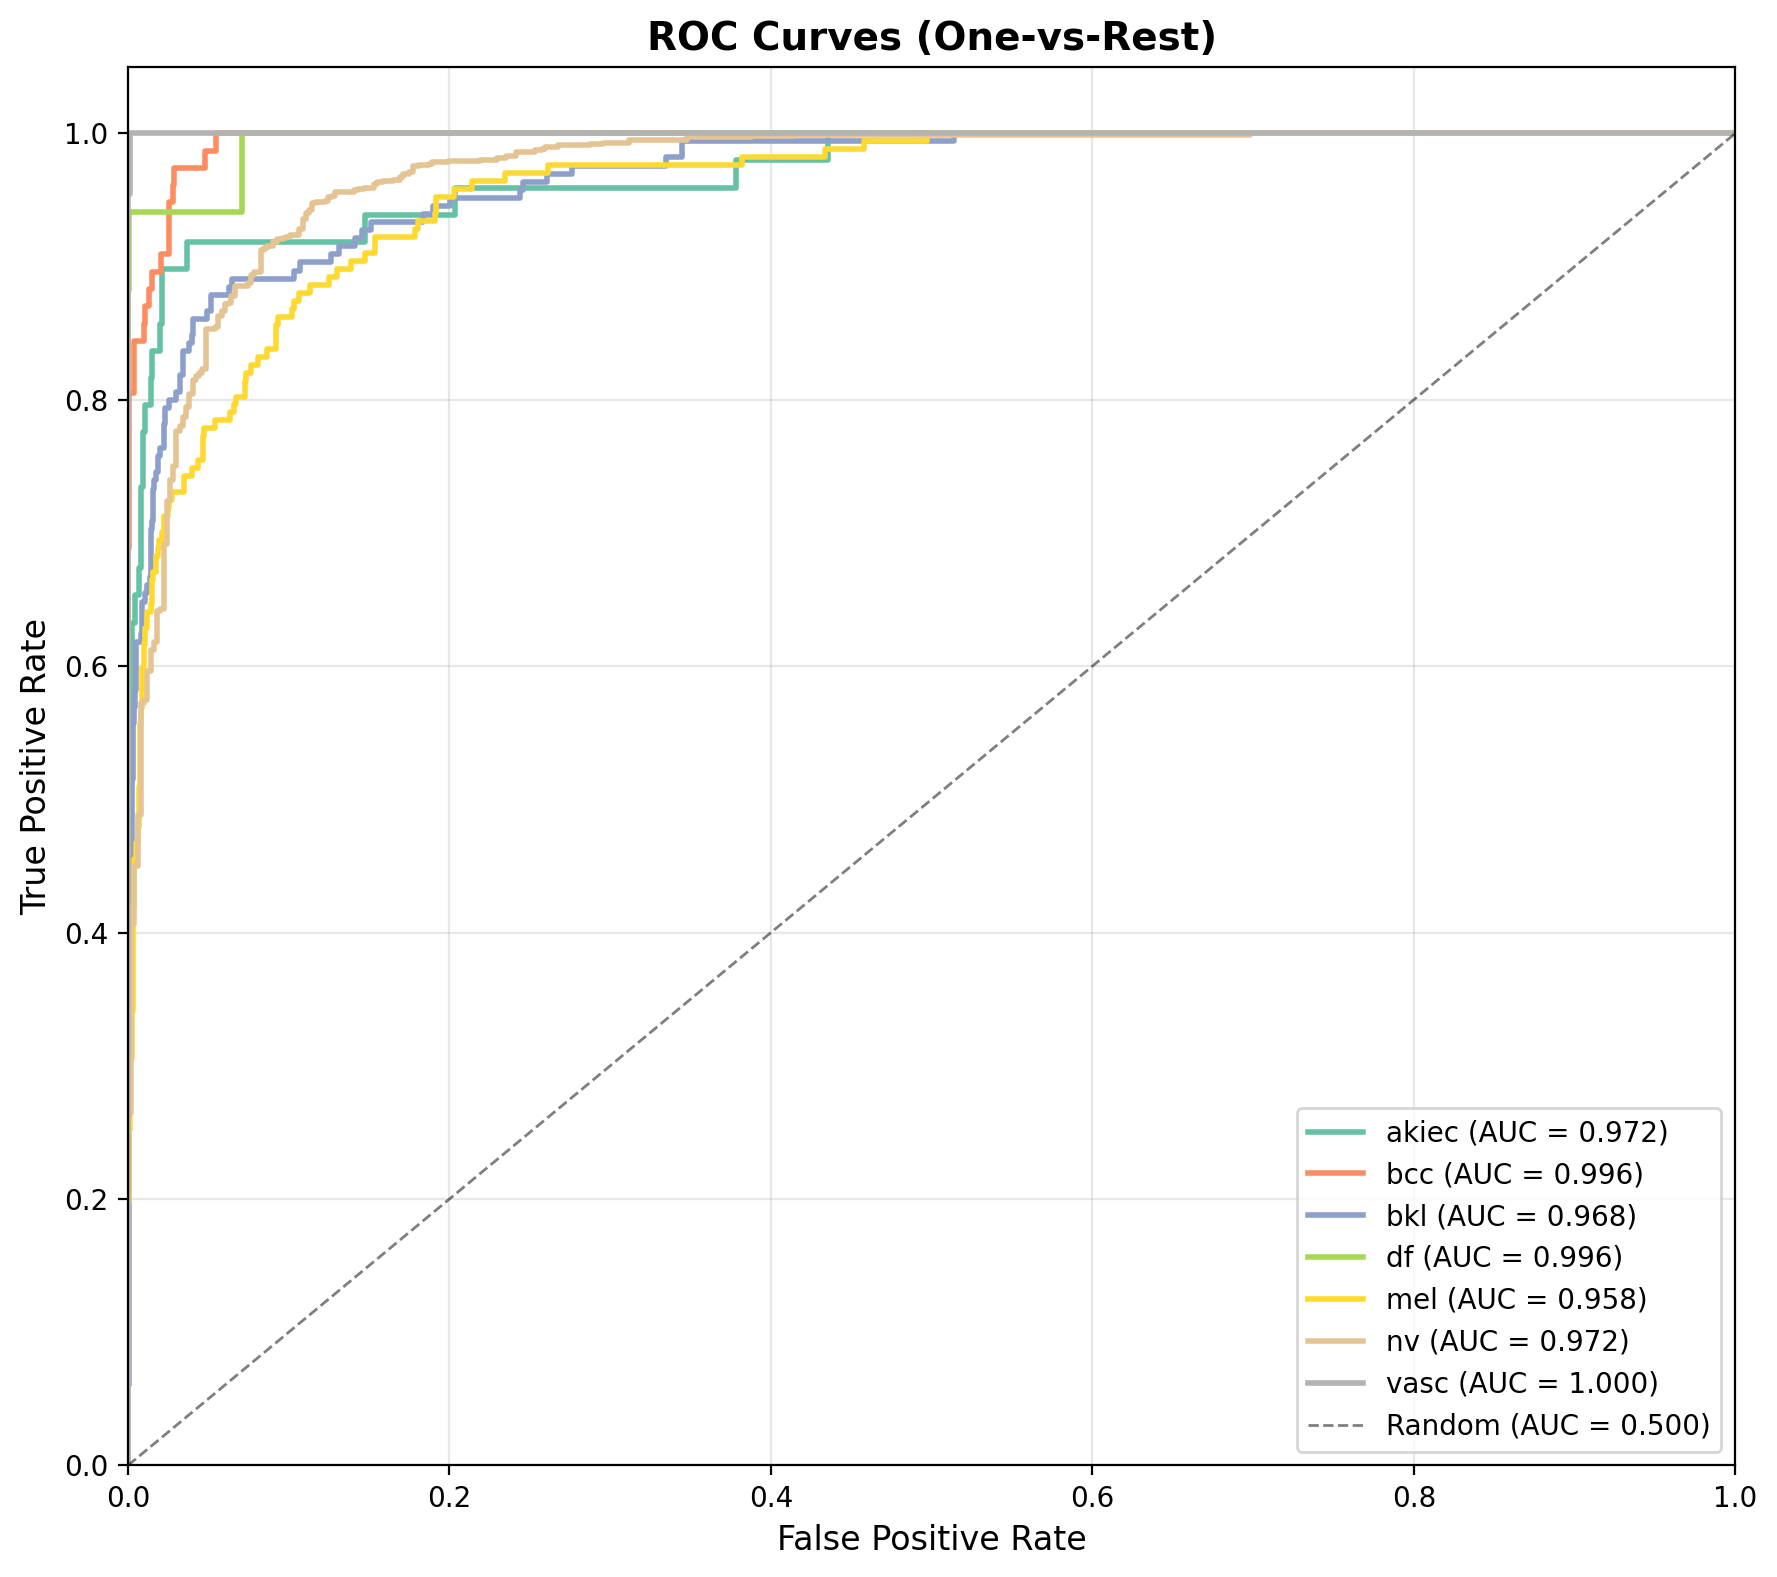
\includegraphics[width=\textwidth]{figures/ensemble_roc_curves.png}
    \caption{ROC curves}
\end{subfigure}
\caption{Ensemble model performance: (a) normalized confusion matrix and (b) per-class ROC curves with AUC values.}
\label{fig:ensemble_results}
\end{figure}

Table~\ref{tab:ensemble_per_class} shows the per-class ensemble performance compared to the best individual model.

\begin{table}[H]
\centering
\caption{Per-class performance of the ensemble versus the best individual model (EfficientNet-B0).}
\label{tab:ensemble_per_class}
\begin{tabular}{lcccccc}
\toprule
\textbf{Class} & \textbf{EB0 F1} & \textbf{Ens. F1} & \textbf{$\Delta$F1} & \textbf{EB0 AUC} & \textbf{Ens. AUC} & \textbf{$\Delta$AUC}\\
\midrule
AKIEC & 0.717 & 0.710 & $-$0.007 & 0.921 & 0.972 & +0.051 \\
BCC   & 0.865 & 0.825 & $-$0.040 & 0.984 & 0.996 & +0.012 \\
BKL   & 0.758 & 0.796 & +0.038  & 0.938 & 0.968 & +0.030 \\
DF    & 0.938 & 0.938 &  0.000  & 0.963 & 0.996 & +0.033 \\
MEL   & 0.695 & 0.744 & +0.049  & 0.913 & 0.958 & +0.045 \\
NV    & 0.940 & 0.946 & +0.006  & 0.946 & 0.972 & +0.026 \\
VASC  & 0.905 & 0.955 & +0.050  & 1.000 & 1.000 &  0.000 \\
\bottomrule
\end{tabular}
\end{table}

\section{Grad-CAM Interpretability Analysis}

To verify that the models are making predictions based on clinically relevant features, Grad-CAM heatmaps were generated for all four models on test-set samples. Figure~\ref{fig:gradcam_grid} shows a comprehensive comparison across all seven disease classes.

\begin{figure}[H]
\centering
\includegraphics[width=\textwidth]{figures/gradcam_class_grid.png}
\caption{Grad-CAM heatmap comparison across all seven classes and four models. Red regions indicate high model attention; blue regions indicate low attention. Green titles indicate correct predictions; red titles indicate misclassifications.}
\label{fig:gradcam_grid}
\end{figure}

Key observations from the Grad-CAM analysis:

\begin{itemize}
    \item \textbf{All models consistently focus on the lesion region} rather than surrounding healthy skin, background artifacts, or ruler markings. This confirms that the learned representations are clinically relevant.
    \item \textbf{EfficientNet-B0 produces the most focused heatmaps}, concentrating attention tightly on the lesion boundary---a feature that dermatologists also prioritize when assessing border irregularity.
    \item \textbf{Swin-Tiny exhibits broader attention patterns}, consistent with the global receptive field of self-attention. While this captures the overall shape of the lesion, it may include some non-discriminative surrounding tissue.
    \item \textbf{For melanoma samples} (Figure~\ref{fig:gradcam_mel}), all models attend to areas of asymmetric pigmentation and irregular borders, which align with the ABCDE criteria used in clinical dermatology (Asymmetry, Border irregularity, Color variation, Diameter, Evolution).
\end{itemize}

\begin{figure}[H]
\centering
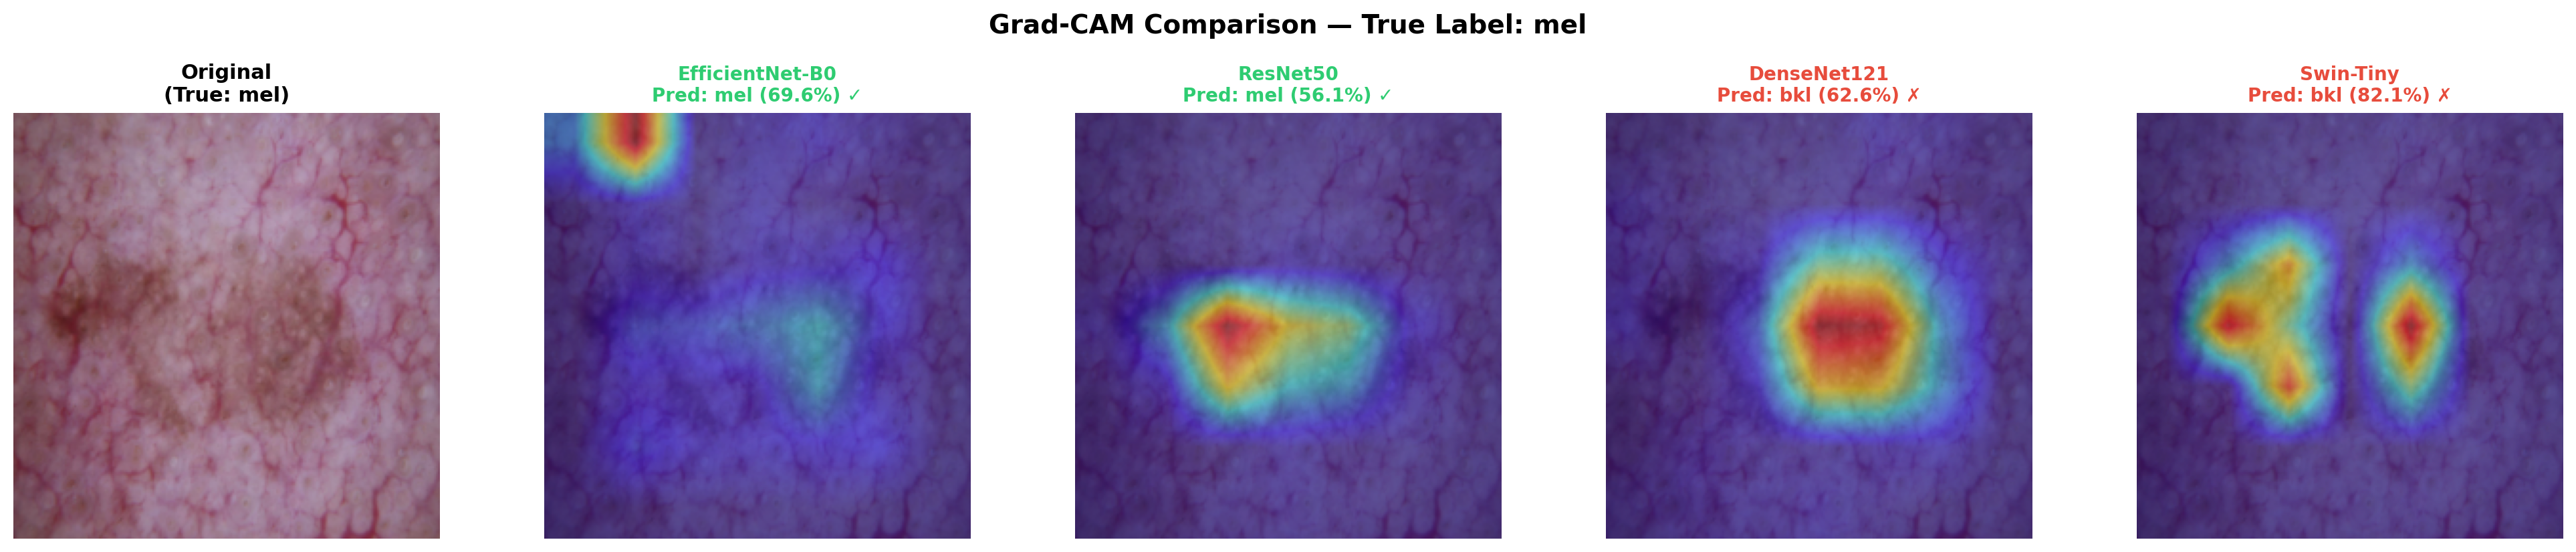
\includegraphics[width=\figwidth]{figures/gradcam_mel_sample.png}
\caption{Grad-CAM visualization for a melanoma sample. All four models correctly focus on the irregularly pigmented lesion area.}
\label{fig:gradcam_mel}
\end{figure}

\section{Ablation Study}

To quantify the contribution of each component in our training pipeline, an ablation study was conducted using EfficientNet-B0 as the base model. In each experiment, a single component was removed while keeping all others fixed.

\begin{table}[H]
\centering
\caption{Ablation study results on EfficientNet-B0. Each row shows the effect of removing one component from the full pipeline. $\Delta$ indicates the change relative to the full model.}
\label{tab:ablation}
\begin{tabular}{lccccc}
\toprule
\textbf{Configuration} & \textbf{Accuracy} & \textbf{Macro F1} & \textbf{AUC} & \textbf{Kappa} & \textbf{$\Delta$ Macro F1}\\
\midrule
Full Pipeline (baseline) & \textbf{0.8836} & \textbf{0.8311} & 0.9522 & \textbf{0.7710} & --- \\
\midrule
$-$ Mixup / CutMix       & 0.8589 & 0.7860 & 0.9486 & 0.7383 & $-$0.0451 \\
$-$ Weighted Sampler     & 0.8762 & 0.8041 & 0.9521 & 0.7487 & $-$0.0270 \\
$-$ Label Smoothing      & 0.8776 & 0.8000 & 0.9674 & 0.7568 & $-$0.0311 \\
$-$ Advanced Augmentation& 0.8896 & 0.8204 & \textbf{0.9664} & 0.7772 & $-$0.0107 \\
\bottomrule
\end{tabular}
\end{table}

The ablation results presented in Table~\ref{tab:ablation} provide strong empirical justification for the proposed training pipeline. The key findings are:

\textbf{Mixup and CutMix are the most critical components.} Removing these spatial and label-mixing regularizations~\cite{zhang2018mixup,yun2019cutmix} resulted in the most severe performance degradation, causing a massive drop of 4.5\% in Macro F1. Without the synthetic examples generated by Mixup and CutMix, the model quickly memorized the rare classes during training and failed to generalize to the test set, leading to early overfitting.

\textbf{Label Smoothing prevents overconfidence.} Removing Label Smoothing~\cite{szegedy2016rethinking,muller2019does} caused a 3.1\% drop in Macro F1. Interestingly, removing label smoothing \textit{increased} the AUC from 0.952 to 0.967, suggesting that while label smoothing improves hard classification decisions by preventing overconfident predictions, it slightly reduces the sharpness of the probability ranking. In skin lesion classification, borders between classes like Melanoma and Nevi are highly ambiguous. Label smoothing acts as a soft margin, preventing the model from becoming overly confident in ambiguous predictions and improving the separation of classes.

\textbf{Weighted Random Sampler is essential for minority classes.} Removing the weighted sampler~\cite{buda2018systematic} led to a 2.7\% drop in Macro F1. Without it, the model prioritized the heavily dominant Nevi class (which accounts for over 60\% of the dataset) at the expense of rare but critical classes like Dermatofibroma and Vascular Lesions.

\textbf{Advanced Augmentations slightly hurt Accuracy but improve F1.} Interestingly, removing advanced augmentations~\cite{shorten2019survey} (such as RandomResizedCrop, Gaussian Blur, and Random Erasing~\cite{zhong2020random}) actually increased raw Accuracy to 88.96\% but decreased the Macro F1 score by 1.07\%. This highlights the tradeoff in imbalanced datasets: aggressive augmentation makes the training task harder, slightly reducing the accuracy on the easy majority class, but significantly improves the model's robustness on the harder, less-represented classes.

% ======================= CHAPTER 5: CONCLUSION ==========================
\chapter{Conclusion and Future Work}

\section{Summary of Contributions}

This thesis presented a systematic comparative evaluation of four deep learning architectures for multi-class skin lesion classification on the ISIC 2018 dataset. The key contributions of this work are:

\begin{enumerate}
    \item \textbf{An optimized training pipeline} that effectively addresses the severe class imbalance (58:1 ratio) inherent in dermatological datasets through a combination of Weighted Random Sampling, Mixup, CutMix, and Label Smoothing. This pipeline demonstrated consistent effectiveness across all four architectures, eliminating overfitting in every case.
    
    \item \textbf{A comprehensive architectural comparison} spanning three CNN families (EfficientNet-B0, ResNet50, DenseNet121) and one Vision Transformer (Swin-Tiny). The results revealed that EfficientNet-B0 achieves the best individual performance (88.36\% accuracy, 0.831 macro F1) with the fewest parameters (5.3M), while Swin-Tiny provides the best probability calibration (0.960 AUC) but suffers from limited data availability.
    
    \item \textbf{A soft-voting ensemble} that leverages architectural diversity to boost performance to 89.49\% accuracy and 0.980 macro AUC, surpassing all individual models and demonstrating the complementary nature of CNNs and Transformers.
    
    \item \textbf{Grad-CAM interpretability analysis} confirming that all models attend to clinically relevant lesion features, a critical requirement for any AI system intended for medical deployment.
    
    \item \textbf{An ablation study} quantifying the individual contribution of each regularization technique, providing empirical evidence for the design decisions underlying the pipeline.
\end{enumerate}

\section{Key Findings}

The experimental results yielded several insights with practical implications:

\textbf{Efficiency matters:} EfficientNet-B0, despite being 5$\times$ smaller than ResNet50 and Swin-Tiny, consistently outperformed them on hard-classification metrics. This challenges the notion that larger models necessarily produce better results, particularly in data-constrained medical imaging scenarios.

\textbf{CNNs vs. Transformers:} An interesting inverse relationship was observed between accuracy and AUC across the four models. CNNs (particularly EfficientNet) excelled at discrete classification, while the Transformer (Swin-Tiny) produced better-calibrated probabilities. This suggests that in clinical applications where probability ranking is more important than binary decisions (e.g., triage systems), Transformers may be preferred despite lower accuracy.

\textbf{Melanoma remains the hardest class:} Across all models and the ensemble, melanoma (MEL) consistently achieved the lowest F1-scores, reflecting the genuine clinical difficulty of distinguishing early-stage melanoma from benign nevi. This highlights the need for continued research into melanoma-specific feature learning.

\textbf{Ensembles are effective:} The simple averaging of probability distributions from four models provided a meaningful improvement across all metrics, with the most notable gain in AUC (+2.8\%). This improvement comes at no additional training cost, requiring only inference from multiple models.

\section{Limitations}

This study has several limitations that should be acknowledged:

\begin{itemize}
    \item \textbf{Single dataset:} All experiments were conducted on ISIC 2018. Cross-dataset evaluation on ISIC 2019/2020 or private clinical datasets would strengthen the generalizability claims.
    \item \textbf{Fixed image resolution:} All models used $224 \times 224$ input resolution. Higher resolutions (e.g., $384 \times 384$) may capture finer details relevant for subtle lesions but would increase computational cost.
    \item \textbf{No external clinical validation:} The models were not evaluated by practicing dermatologists in a clinical workflow, which would be necessary before any real-world deployment.
    \item \textbf{Limited Transformer exploration:} Only Swin-Tiny was evaluated. Larger Swin variants or other ViT architectures (e.g., DeiT, BEiT) might perform differently.
\end{itemize}

\section{Future Work}

Several promising directions for future research emerge from this study:

\begin{itemize}
    \item \textbf{Web-based deployment:} Develop an interactive web application (using Streamlit or Gradio) that allows clinicians to upload dermoscopy images and receive real-time predictions with Grad-CAM visualizations.
    \item \textbf{Test-Time Augmentation (TTA):} Apply multiple augmentations during inference and average the predictions, potentially boosting accuracy by 1--2\% without retraining.
    \item \textbf{Knowledge distillation:} Transfer the knowledge from the ensemble into a single lightweight model suitable for mobile or edge deployment.
    \item \textbf{Self-supervised pretraining:} Leverage large unlabeled dermoscopy image collections to pretrain models using contrastive learning (e.g., SimCLR, DINO) before fine-tuning on the labeled ISIC data.
    \item \textbf{Multi-task learning:} Jointly predict diagnosis and segmentation masks, as lesion boundary information may improve classification accuracy.
\end{itemize}


% ======================= REFERENCES ==========================
\printbibliography[title={References}]

\end{document}
